\chapter{Auroral Energy and Flux Derivation} \label{chap:energy}

In this chapter we will discuss about the background on derivation of auroral electron energy flux using multi-spectral measurement of three prominent upper atmospheric emissions. The OI 630.0 nm (red line), the OI 557.7 nm (green line) and $N_{2}^{+}$ 427.8 nm (blue line) emission brightnesses are compared with model to derive energy and flux.

Energetic electrons are stopped at certain altitudes as they penetrate through the atmosphere based on their initial kinetic energy. This determines the ionization rate and the altitude of ionization peak \citep{rees_1963}. That is, the peak ionization moves to a lower altitude and the ionization rate increases with increasing energy causing the brightness of each emission feature to change differently as a function of energy (see Figure \ref{fig:vve} ). These brightnesses can be estimated using a theoretical electron transport and chemical reaction model and then compared with measurements to derive the primary electron energy and energy flux. 



The GLOW model \citep{solomon_1988}, is a two stream electron transport and chemical reaction model that is capable of estimating the emission from various spectral features based on a modeled neutral atmosphere (MSIS-00, see \citet{msie}), an ionosphere (IRI-90, see \citet{iri}), geophysical parameters and the energy and energy flux of precipitating electrons. The primary precipitating electrons are assumed to have a Maxwellian energy distribution that is characterized by the “characteristic energy” (half of the mean energy) $E_0$ and the characteristic energy flux $Q_0$. The GLOW model also incorporates the contribution to the emission due to solar radiation as well as chemical reactions in the upper atmosphere.  



The GLOW model will be used to estimate the emission strength of the OI 557.7 nm, OI 630.0 nm and  $N_{2}^{+}$  427.8 nm emission features at different input energy and energy fluxes. These input energy and energy flux will then be constrained with emission measurements. The results will be compared to a different method used by Pallamraju et al. 2011 where the authors utilize the OI 630.0 nm emission measurements (from an instrument similar to HiT\&MIS) together with the GLOW model and ISR measurements to estimate the characteristic energy and energy flux due to electron precipitation during a geomagnetic storm \citep{pallamraju_2011}.

\section{Background Literature Review}
% The magnetosphere and the thermosphere-ionosphere system are coupled through the Earth's magnetic field lines allowing solar wind electrons to enter the upper atmosphere of the Earth. Interaction between the precipitating electrons and atmospheric species gives rise to auroral emissions. Auroral electron precipitation is one of the major sources of solar energy input to the upper atmosphere especially at high latitudes where they most commonly occur. The upper atmospheric heating caused by such events can be equal to that caused by solar EUV photons at times \citep{mayr_1978}. Thus, estimating the electron precipitation energy and energy flux during such events allows for better quantification of the energy budget and provides insight into coupling between different atmospheric regions. 
%This allows for  precipitating energy to be deposited at mid and low latitudes.

The energy and energy flux of the primary electrons during auroral precipitation events have in general measured from instruments on board satellites or  from sounding rockets. These include in situ measurements from particle detectors on sounding rockets (\citet{rocket,michell_2016} and references therein) and combined rocket-based in situ particle measurements and ground based multi-spectral measurements \citep{grubbs_multi_spec}. The energy and flux have also been inferred remotely by satellite-based UV measurements (see, for example, \citet{guvi}).
Electron energies and fluxes have also been estimated from the ground using Incoherent Scatter Radar (ISR) \citep{semeter_2005} and combined optical and radar measurements \citep{pallamraju_2011}. In addition, a method for deriving precipitating electron energy fluxes by solving a large linear inversion problem based on multi-wavelength (red and green lines) all-sky imagers was presented by \citet{jan_rcons2001}.

Energetic electrons penetrating into the Earth's atmosphere are stopped at different altitudes based on their initial energies; particles with higher energies penetrate deeper into the atmosphere while those with lower energies are stopped at higher altitudes \citep{rees_1963}.
Thus, the peak height of the electron density profile depends on the energy of precipitating electrons during such events.
Using this concept, \cite{pallamraju_2011} derived energies of the precipitating electrons using the F2 peak heights (hmF2) from nearby ISR measurements for an auroral event over Boston, MA. The energy fluxes were then derived by matching the measured red line brightness to that predicted by a physics-based electron transport model called GLobal airglOW (GLOW) \citep{solomon_1988,solomon1989630,bailey2002}.  

%In that study, however, auroral arcs that were off zenith were smeared out (loss in spatial resolution) as the viewing geometry became oblique. In addition, the images at different wavelengths were not simultaneous and so an auroral feature might be at a different location in each wavelength.
%The authors used the electron density ($N_e$) and electron temperature ($T_e$) profiles from ISR measurements as inputs into the GLOW model.

%Energetic electrons penetrating into the Earth's atmosphere are stopped at different altitudes based on their initial energies. Particles with higher energies penetrate deeper into the atmosphere while those with lower energies are stopped at higher altitudes \citep{rees_1963}.
%This causes the peak height of the $N_e$ profile to depend on the energy of precipitating electrons during such events.

%Various mechanisms of emission production, such as electron impact excitation and dissociative recombination, depend on the interaction between the atmospheric species and electrons, and hence the electron density profile. Furthermore, p

Particular emissions peak around certain altitudes based on their production mechanism (including collision involving incident electrons) and the density of the atmospheric species producing the emission. Therefore, the column brightness of each emission feature is sensitive to the changes in electron density around the altitude of its peak production. This means that during aurorae, each emission feature responds differently to a given energy distribution of precipitating electrons. %Thus, retrival of energy and flux of precipitating electrons using multi-spectral measurements have been explored previously.
Simultaneous measurements of multiple emission features therefore allows for the energy and flux of the precipitating electrons to be inferred. \citet{rees_1974} explored the theoretical relationship between the ratios of auroral contributions to the $N{_2}{^+}$ (427.8 nm, blue line), OI (557.7 nm, green line) and OI (630.0 nm, red line) column brightnesses to infer the incident electron energy. The absolute column brightness of the blue line was used by the authors to deduce the total flux. Similar to \citet{rees_1974}, \citet{grubbs_compare} used the ratio of OI 844.6 nm to green line and the blue line brightness to derive energy and flux for an auroral event.

During certain geomagnetic storms the z-component of the Interplanetary Magnetic Field (IMF), $B_z$, turns southward (negative) and the auroral oval extends equatorward (\citet{holzworthmeng,hardy}, etc.). Such was the case during the June 22-23, 2015 G4 storm, where the extended auroral oval produced emissions observed in Lowell, MA (42$^\circ$N, 71$^\circ$W: Geographic, 52$^\circ$N: Geomagnetic Latitude) by a ground-based imaging spectrograph. In this paper, we explore the feasibility of using column brightnesses and brightness ratios of red, blue and green emission lines to simultaneously derive energy and flux of precipitating electrons by constraining the GLOW model estimation with the measurements made on June 22-23, 2015. In addition, a hybrid method using brightness ratios to derive energy and brightnesses to derive fluxes similar to \cite{rees_1974} is also applied for comparison. The spatial and temporal morphologies of the derived energies and energy fluxes during the June 22-23, 2015 G4 storm are then discussed.

\section{Observations}
We observed an auroral event from Lowell, MA on June 22-23, 2015 using the High Throughput and Multi-slit Imaging Spectrograph (HiT\&MIS) \citep{hitmis}. This event was triggered by a G4 storm which itself was associated with an X-class solar flare. Earth's geomagnetic field was disturbed in the process such that the minimum
value for the Dst index reached -204 nT \citep{baker_dst}.

HiT\&MIS has a field of view (FOV) of 0.1$^\circ$ by 50$^\circ$. Observations were made with its FOV centered at a geographic Zenith Angle (ZA, angle from the Zenith) of 45$^\circ$, pointing towards the northeast, with the length of the 50$^\circ$ FOV in N-S direction (Figure \ref{fig:elayer}). Measurements were taken with a cadence of
70 seconds (60 seconds exposure time) from 9:30 PM  June 22, 2015 to 4 AM June 23, 2015 (all times given in Local Time (LT)). 

During the observation period the sky was partly cloudy. We use the NeI (630.5 nm) emission feature (also observed by HiT\&MIS) which is produced by street lights as a tracer of cloud activity. We considered only periods with minimal cloud coverage for our analysis (see Figure \ref{feature:nbrg}). 

HiT\&MIS is capable of measuring six upper atmospheric 
emission features simultaneously at high spectral resolution ($\approx$ 0.02 nm at 630.0 nm).
The spectral images were recorded using an ANDOR iKon-M CCD camera cooled to -59$^\circ$ C. To characterize the CCD, the bias frame and the dark frame were obtained by
taking images with varying exposure times while the shutter was closed. Data counts (in Arbitrary Data Unit, ADU) on each pixel were then fitted to a linear equation to estimate the bias and the dark frames. The bias frame was subtracted from each raw image (Figure \ref{fig:raw}A) but the dark frame was negligible ($\approx{}$ 0.0019 ADU $\rm s^{-1} pixel^{-1}$; red line intensity was $\approx$ 10-30 ADU $\rm s^{-1} pixel^{-1}$ for comparison) and hence ignored.

\section{Data and data analysis}
For this study, we used three spectral features observed by HiT\&MIS: blue line, green line and red line. HiT\&MIS creates spectral images of emissions as a function of wavelength and zenith angle (Figure \ref{fig:raw}A). For each spectral feature, we extracted the emission region over a narrow range of wavelength ($\approx$ $\pm$0.3 nm from the line center) from the image. Then, the curvature in the measured spectrum as a function of zenith angle due to the slit geometry was corrected. Finally, the background was estimated by averaging values on both side of the spectral feature and subtracted from the data.
%This gave us the spectral signal (S), the background (B) and the readout noise (RN, standard deviation of the bias frame). 
%The background subtracted spectra (uncalibrated) was now represented as: $S \pm \sqrt{(S+B) + RN^2}$. 

A C-14 activated light source was used to calibrate the signal photometrically (in Raleigh $\rm {\AA}^{-1}$, see Figure \ref{fig:raw}B). The calibrated spectra were averaged over different look direction bins (see Figure \ref{fig:raw}C) to obtain a representative spectrum. Integrating the spectrum along the wavelength axis gives the line of sight brightness at different look directions. The brightness data from HiT\&MIS used for this work are available online at https://doi.org/10.5281/zenodo.1208111.

\subsection{Brightness Morphology} 
\label{sec:bmorph}
To assess the morphology of the emission as a function of time, we divided the data into three look directions (20-37$^\circ$, 37-54$^\circ$ and 54-70$^\circ$ zenith angles). We also selected eight time ranges with minimal cloud coverage for our analysis (labeled T1-T8).
Figure \ref{feature:nbrg} shows the brightnesses for the three spectral features (plus the NeI cloud indicator) as a function of time at different look direction bins. During the time period T1, the brightness are lower at higher zenith angles for the all of the emission features. In contrast, during the time periods T3, T4 and T8 the red line brightnesses are higher at higher zenith angles (Figure \ref{feature:nbrg}). For these three cases, the brightnesses in the other features do not change significantly with change in zenith angle. The auroral red line emission occurs at higher altitude ($\approx$  250 km) and thus spans larger latitude ranges than the blue and green lines (Figure \ref{fig:elayer}). Since this effect is larger for higher zenith angles (north, see Figure \ref{fig:elayer}) we could have been looking at different auroral structure in red line for time periods T3, T4 and T8. 
%  This should have also been visible for the OI (777.4 nm) emissions as it peaks at even higher altitude, but it is not apparent in the poor signal to noise ratio data. 

In the time period T2, the red and the green line brightnesses were relatively constant with time and zenith angles but a few small peaks can be seen in the blue line brightness (see T2 in Figure \ref{feature:nbrg}), particularly at the 37-54$^\circ$ zenith angle look direction. 
There was a decrease in the red line brightness during time period T5, with a few small peaks in the green and blue lines. During the time period T6, all the emission brightnesses were increasing with time, but the increase in the red line was more prominent than other features. These different temporal and angular morphologies in brightnesses provide an opportunity to examine their implications on energies and fluxes are discussed in section \ref{sec:emorph}.
% in conjunction with the morphologies in energies and fluxes. 

% These average brightnesses were the measured data points used for energy and flux derivation for their particular look directions bins (see Figure \ref{feature:nbrg}). This paper describes the methods we used to estimate energies and energy fluxes during the time intervals T1 through T8 in Figure \ref{feature:nbrg} for three look directions. 

%Since the peak emission height of each of the features is different, the measurements represent different latitudes as shown in Figure \ref{fig:elayer} (do we need this part?).
\begin{figure}[hp]
	\centering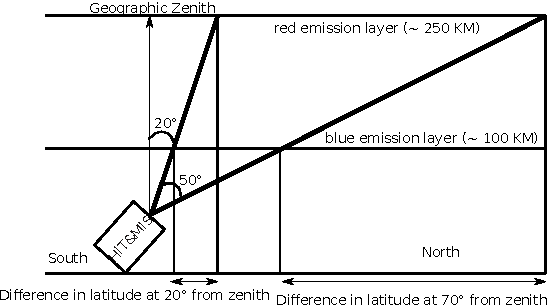
\includegraphics[width=40pc]{elayer.pdf}
	\caption{Viewing geometry of the HiT\&MIS instrument during the June 22-23, 2015 storm at Lowell, MA. The latitudes traced by the red and the blue lines are shown assuming the peak emission height of
		250 km and 100 km, respectively. Note that for measurements closer to the zenith the range of latitudes covered by each emission layer is small. However for measurements far away from the zenith, emissions from a larger latitude range are measured along the line of sight.}
	\label{fig:elayer}
\end{figure}
%%%%
\begin{figure}
	\centering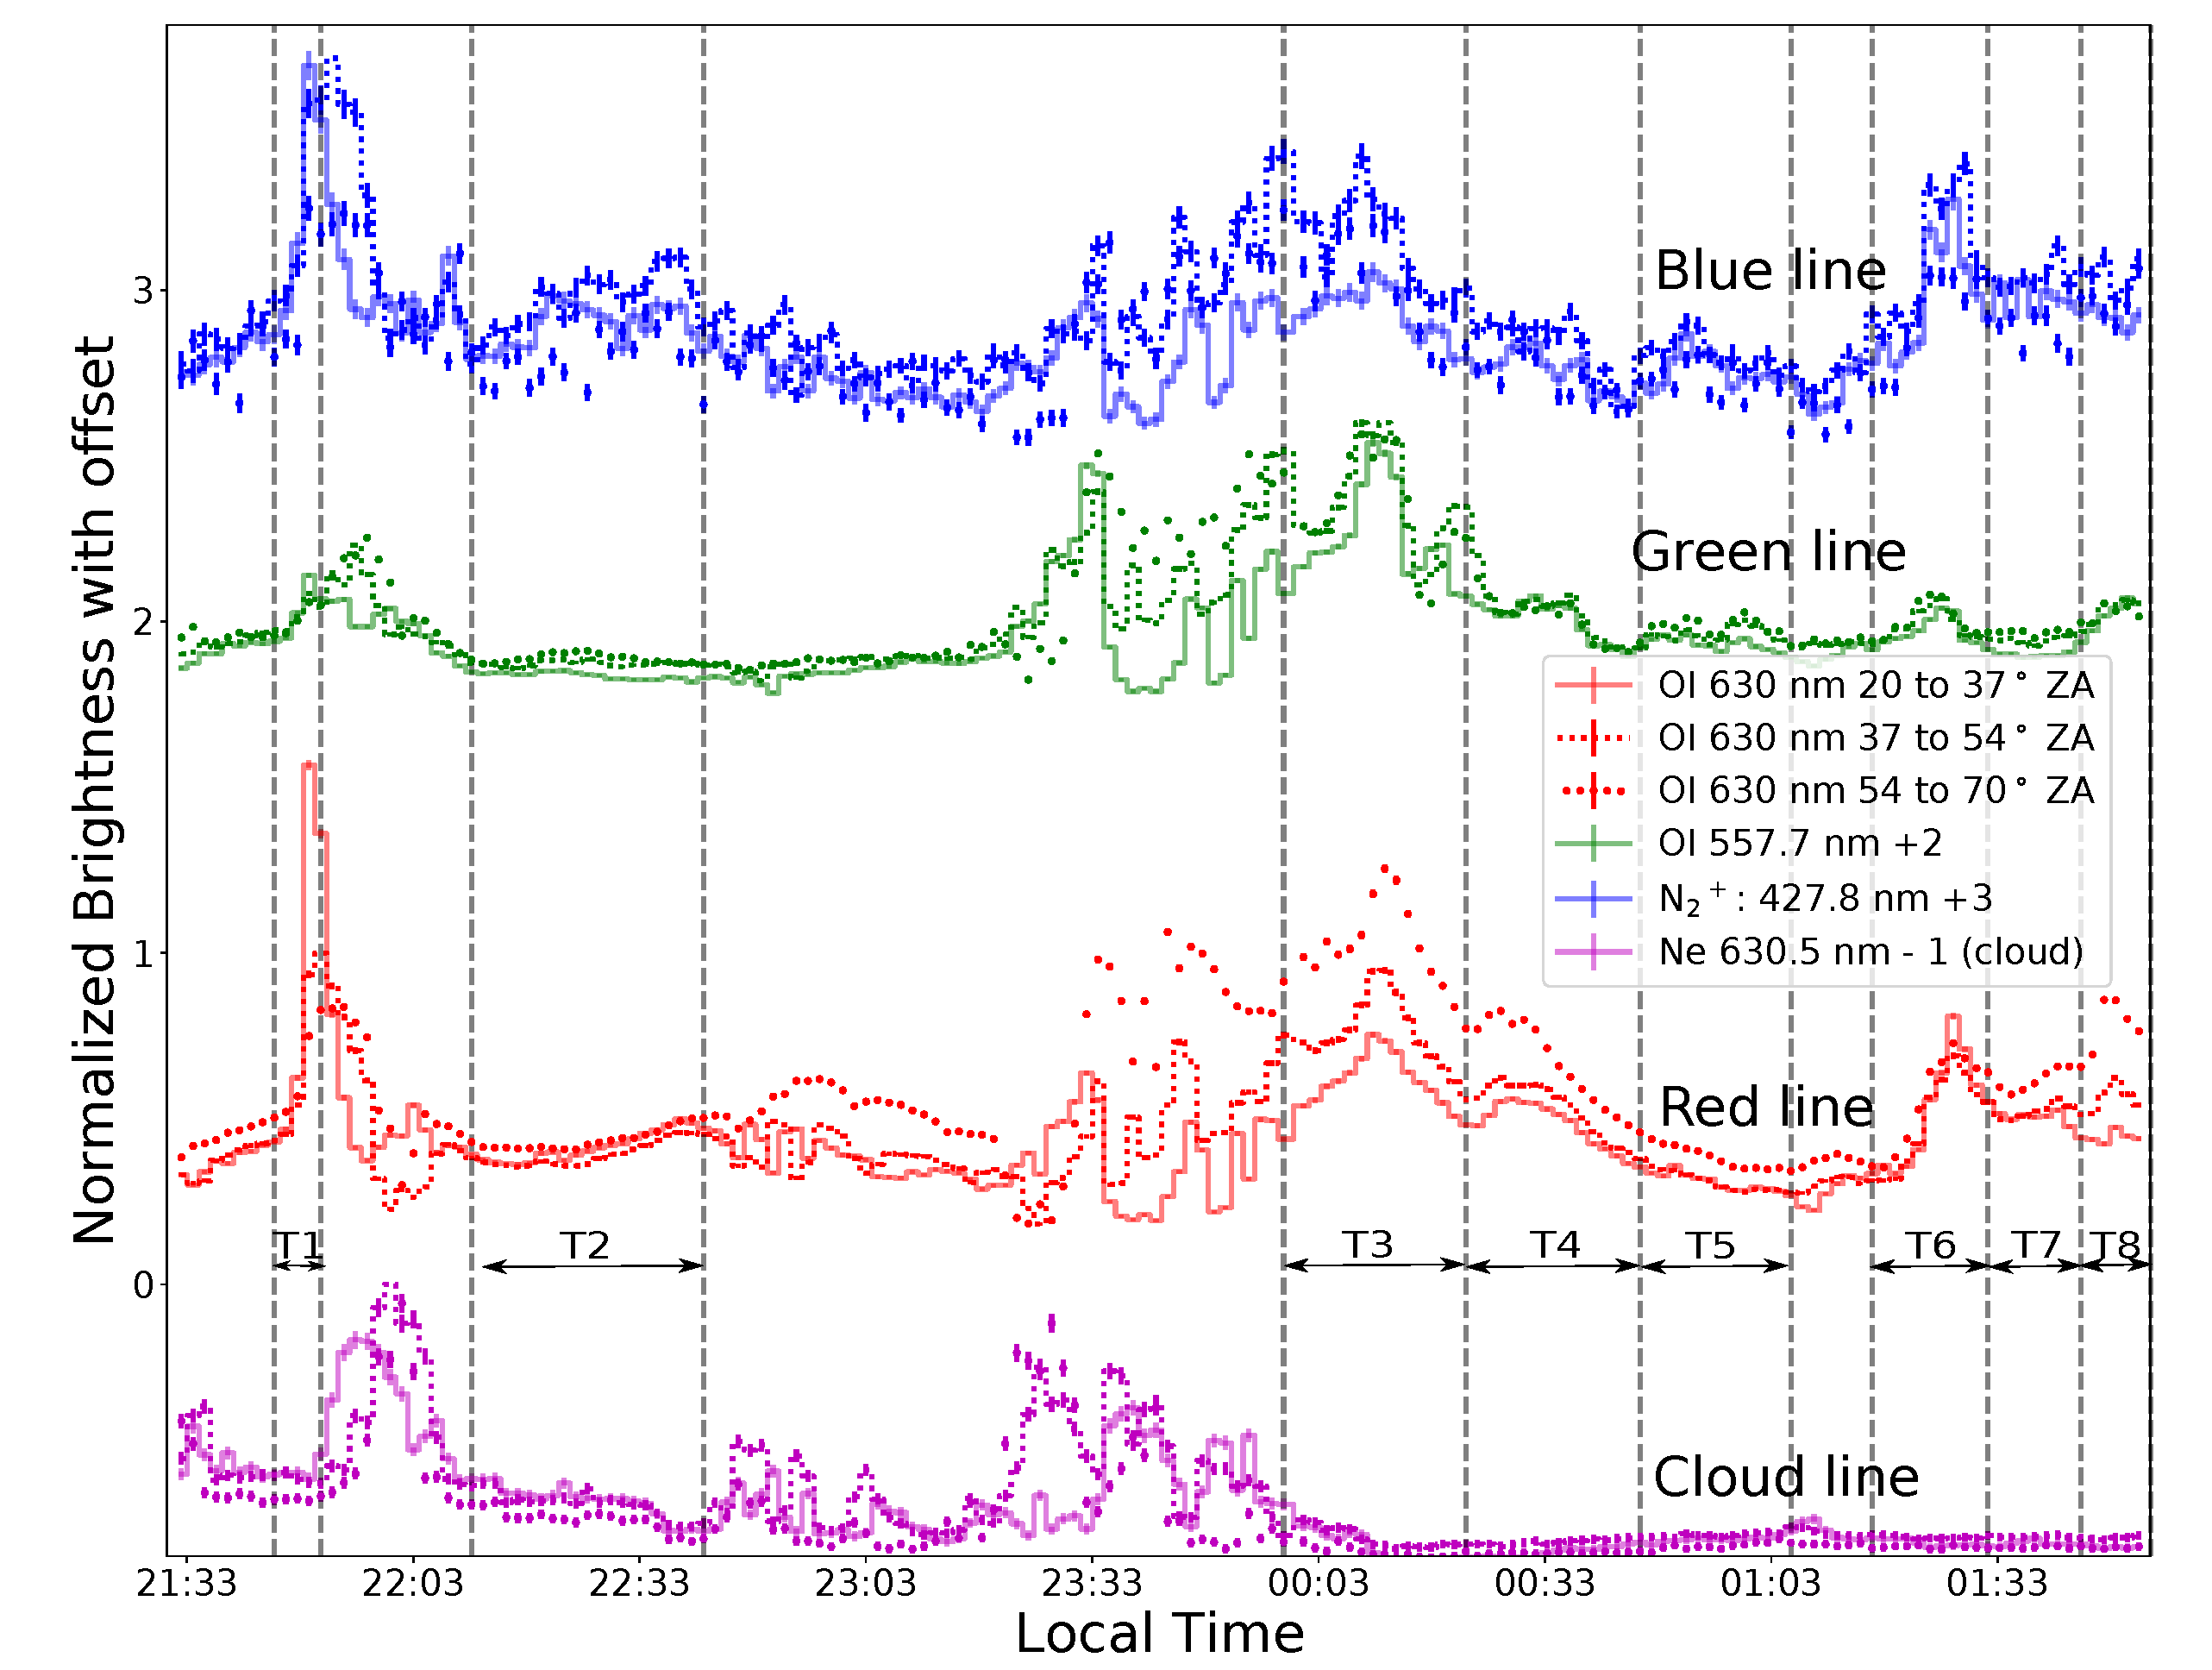
\includegraphics[width=42pc]{nbgr.pdf}
	\caption{Normalized brightness of the four emissions observed with HiT\&MIS through the night of June 22-23, 2015 obtained by averaging along: 20 to 37$^\circ$ (solid line), 37 to 54$^\circ$ (dashed line) and 54 to 70$^\circ$ (dotted line) zenith angles with 60s exposure time. The Ne I (630.5 nm) emissions, used as proxy for cloud activity, is shown in magenta.  
		The emission lines have offsets added to them for clarity. For example, the the green line emission brightness values have an offset of 2 added. The $\pm$1$\sigma$ uncertainties are shown as vertical error bars, which are most prominently seen in the blue line emission brightness.
		The times with minimal cloud activity chosen for analysis are shown with dashed vertical lines and labeled T1 through T8.}
	\label{feature:nbrg}
\end{figure}
%%%%%%
\begin{figure}[hp]
	\centering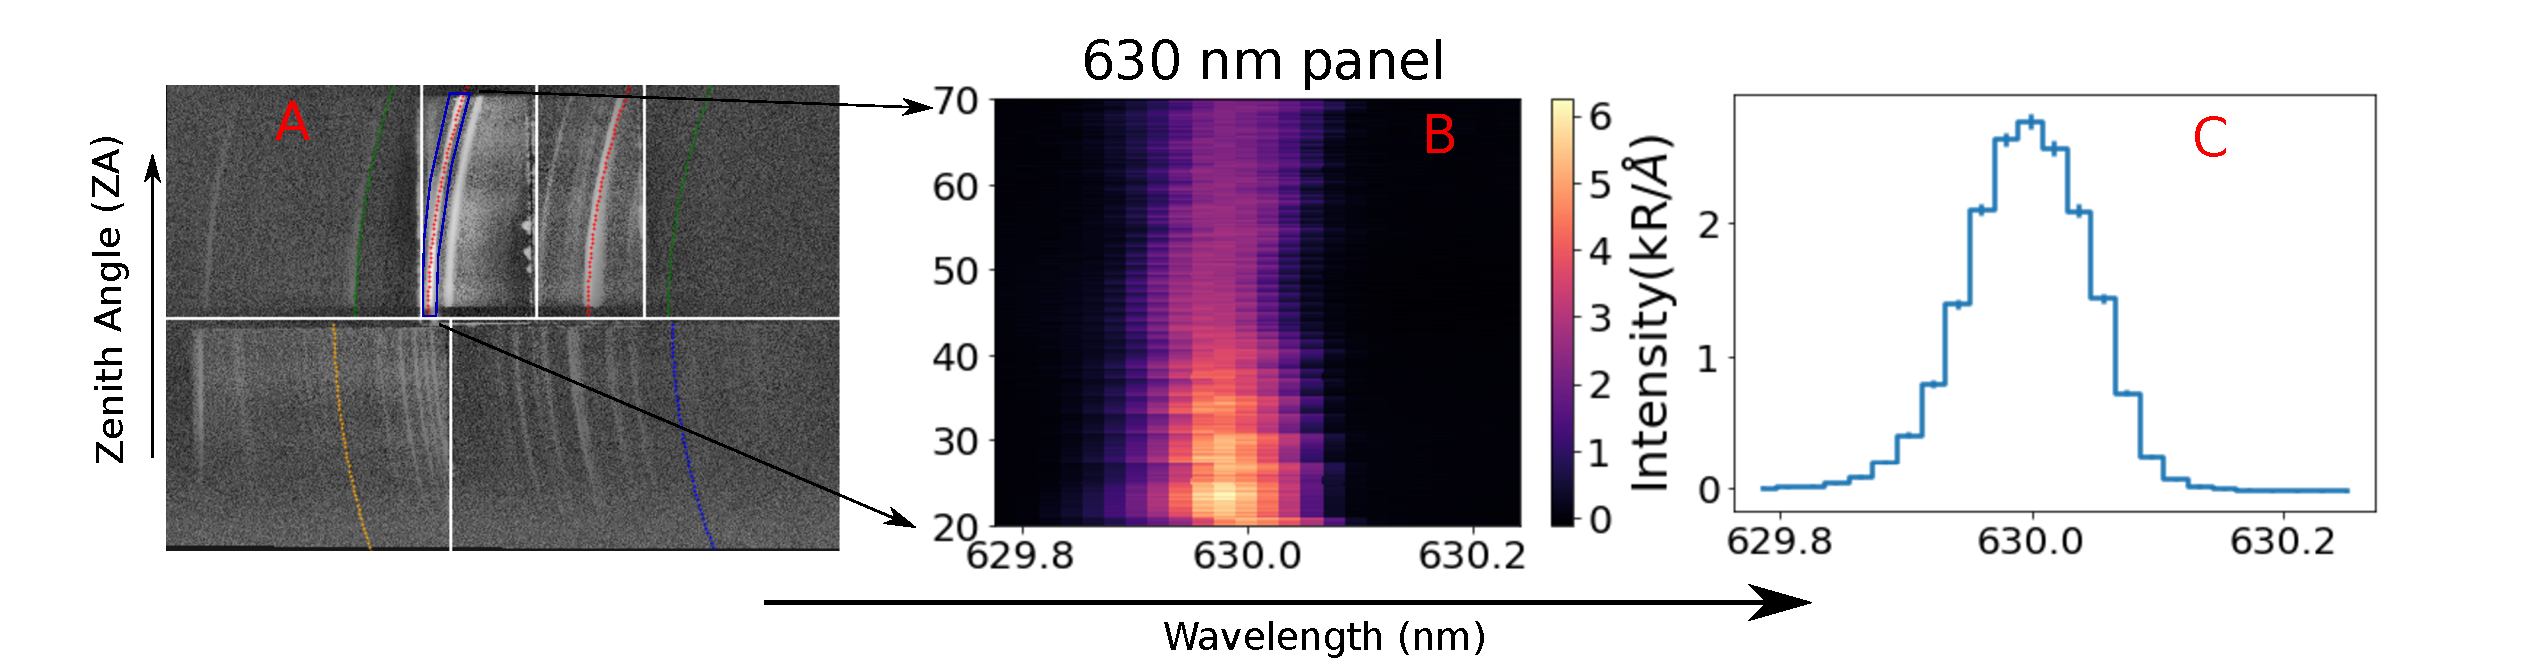
\includegraphics[width=40pc]{raw_spec.pdf}
	\caption{A: Sample raw image from HiT\&MIS at 22:30 PM LT on June 22, 2015 with 60 s exposure. Overlaid lines are the ray trace estimate of the line center locations of the emission features. B: Photometrically calibrated, background-subtracted 630.0 nm spectrum extracted from the region highlighted in A. C: Average spectrum obtained by integrating over 
		over the entire zenith angle range (y-axis in B) covered by HiT\&MIS.}
	\label{fig:raw}
\end{figure}

\section{Modeling} 
\label{sec:model}
The GLOW model is based on a two stream electron transport method of \citet{nagybanks1970}. We assumed that the primary precipitating electrons have a Maxwellian energy distribution with a characteristic energy ($E_{0}$) and total energy flux ($Q_{0}$). These primary electrons then interact with neutral atmospheric species provided by the climatological neutral atmospheric model, NRLMSIS00 (Naval Research Laboratory Mass Spectrometer Incoherent Scatter 2000) \citep{msie} as they move through the upper atmosphere. The climatological ionospheric model, IRI-90 (International Reference Ionosphere 1990) \citep{iri} provides the electron and ion densities and temperatures for photochemical calculations.

 The altitude profiles for the volume emission rate (VER) of the observed emission features were modeled for different input characteristic energies and fluxes using the GLOW model (Figure \ref{fig:vve}, \ref{fig:bve}). 
We vary the energy and flux inputs into GLOW and integrate along line of sight volume emission rate (VER, Figure \ref{fig:vve}) to estimate brightness.
\subsection{Fluorescence contribution removal}
The output of the GLOW model showed two peaks in the blue line VER profile, one at higher altitude and the other at lower altitude. The emission peak at the higher altitude was due to resonance fluorescence of $N{_2}{^+}$ by solar radiation. Because all of our observation are during nighttime we subtract this contribution due to fluorescence in each model run (including Figure \ref{fig:vve}). 

%For our nighttime observations, this contribution was removed by subtracting the fluorescence contribution to the $N{_2}{^+}$ (427.8 nm) VER profile for each of our model runs.

\begin{figure}
	\centering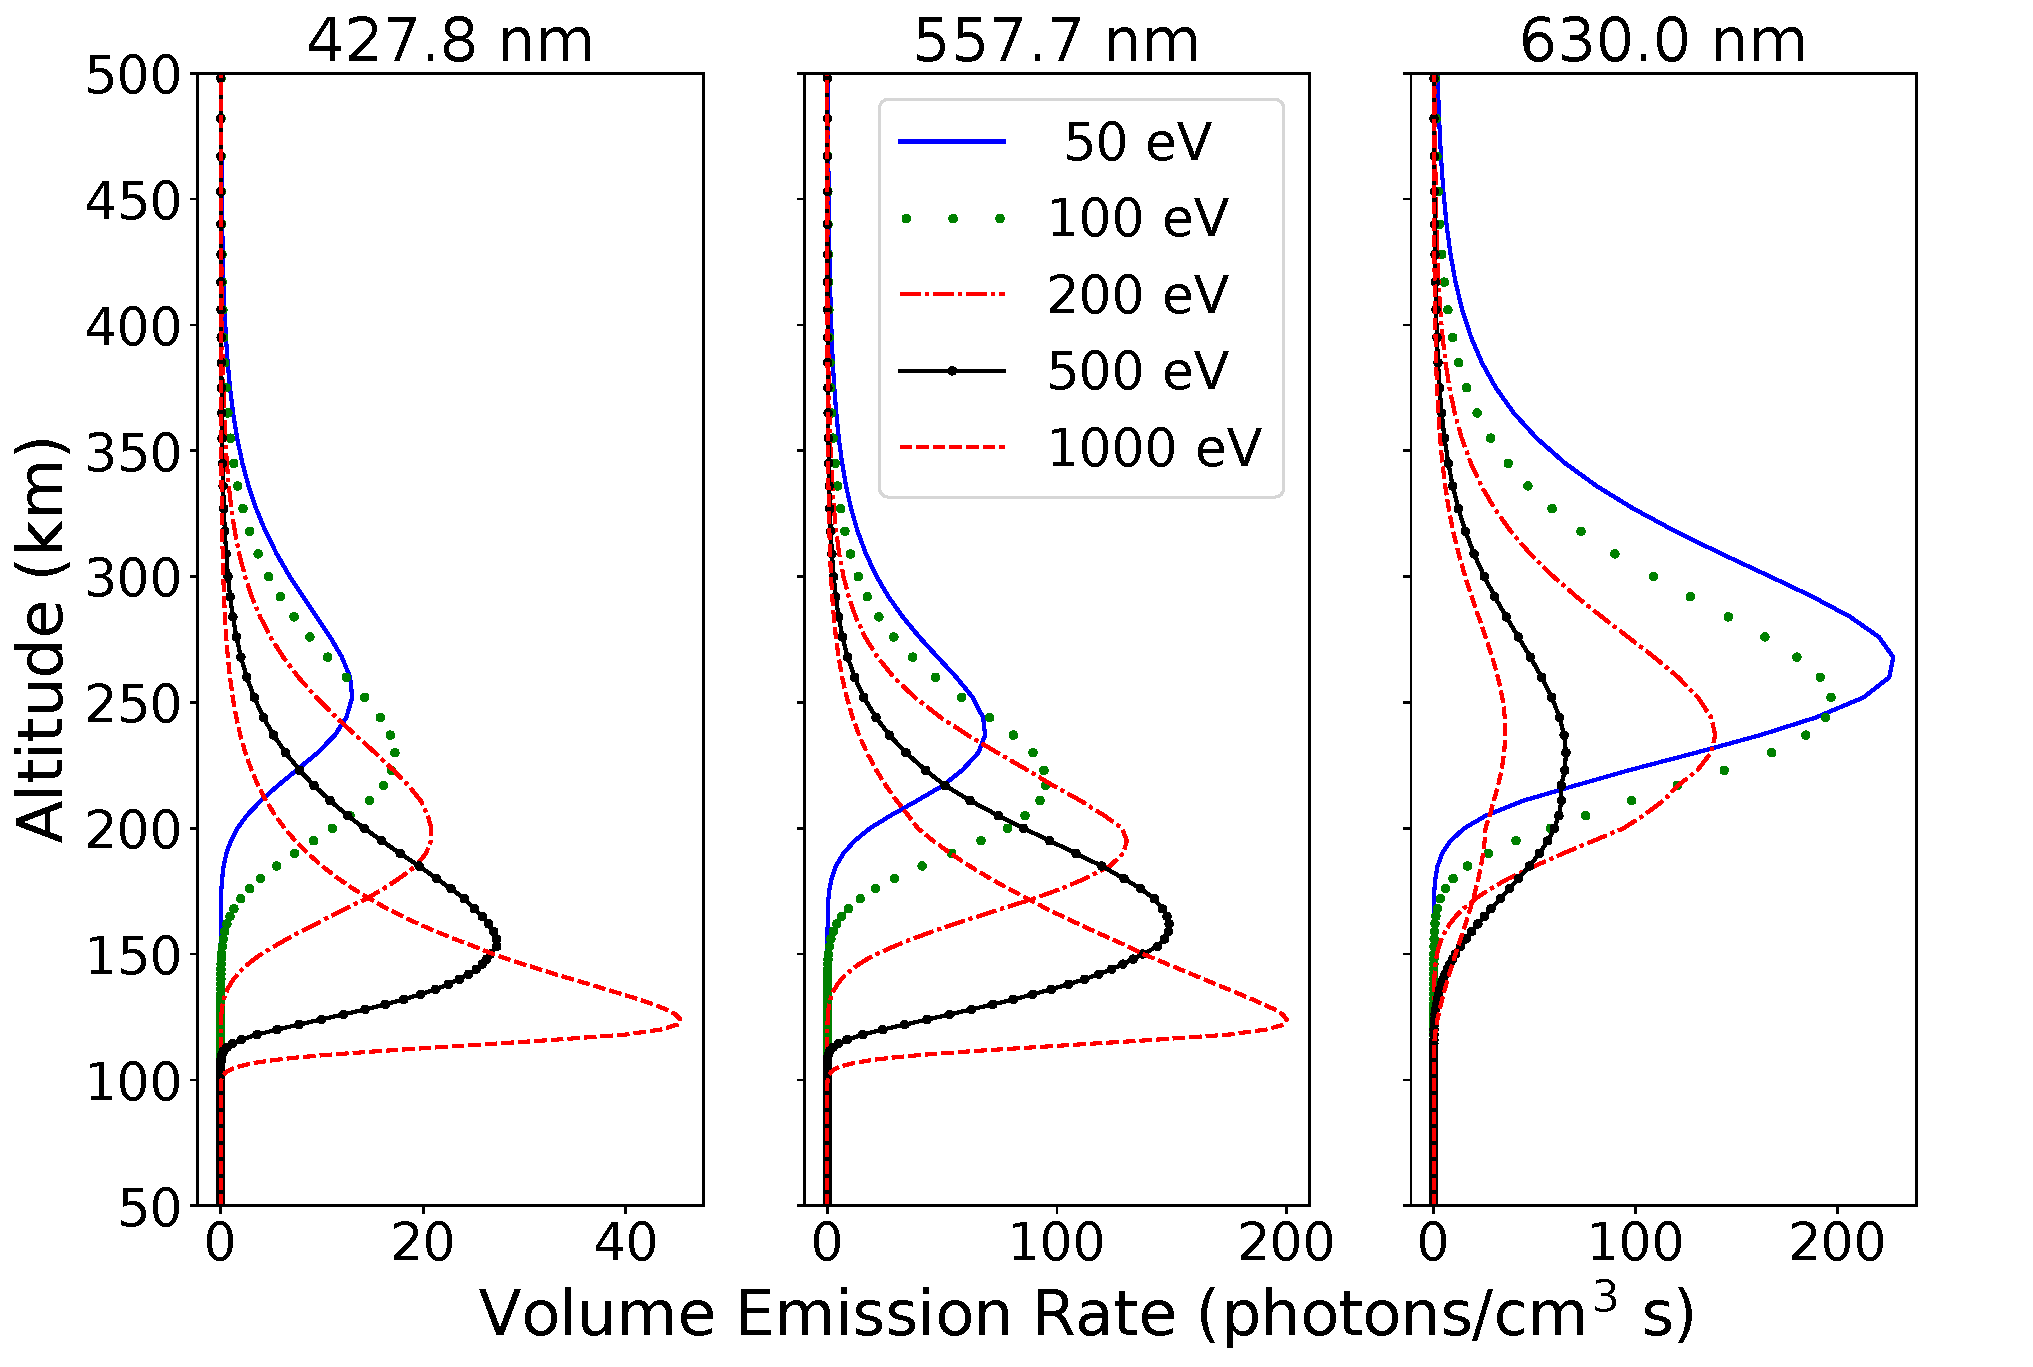
\includegraphics[width=35pc]{ver_vs_e1.pdf}
	\caption{GLOW model volume emission rates with varying energy and a constant flux of 1 erg $\rm cm^{-2}$ $\rm s^{-1}$ computed for the four emission features. Auroral contribution to VER is linearly proportional to flux. Note the peak VER and the altitude of the peak change differently for the different features as a function of energy. For
		example, the peak height for red line (630.0 nm) is around 250 km for all energies and peak VER occurs at less that 100 eV, while the for the blue line (427.8 nm) the peak height is around 100 km and the peak VER occurs in the 1 keV range.}
	\label{fig:vve}
\end{figure}
%%%%%%%%
% \begin{figure}
% \centering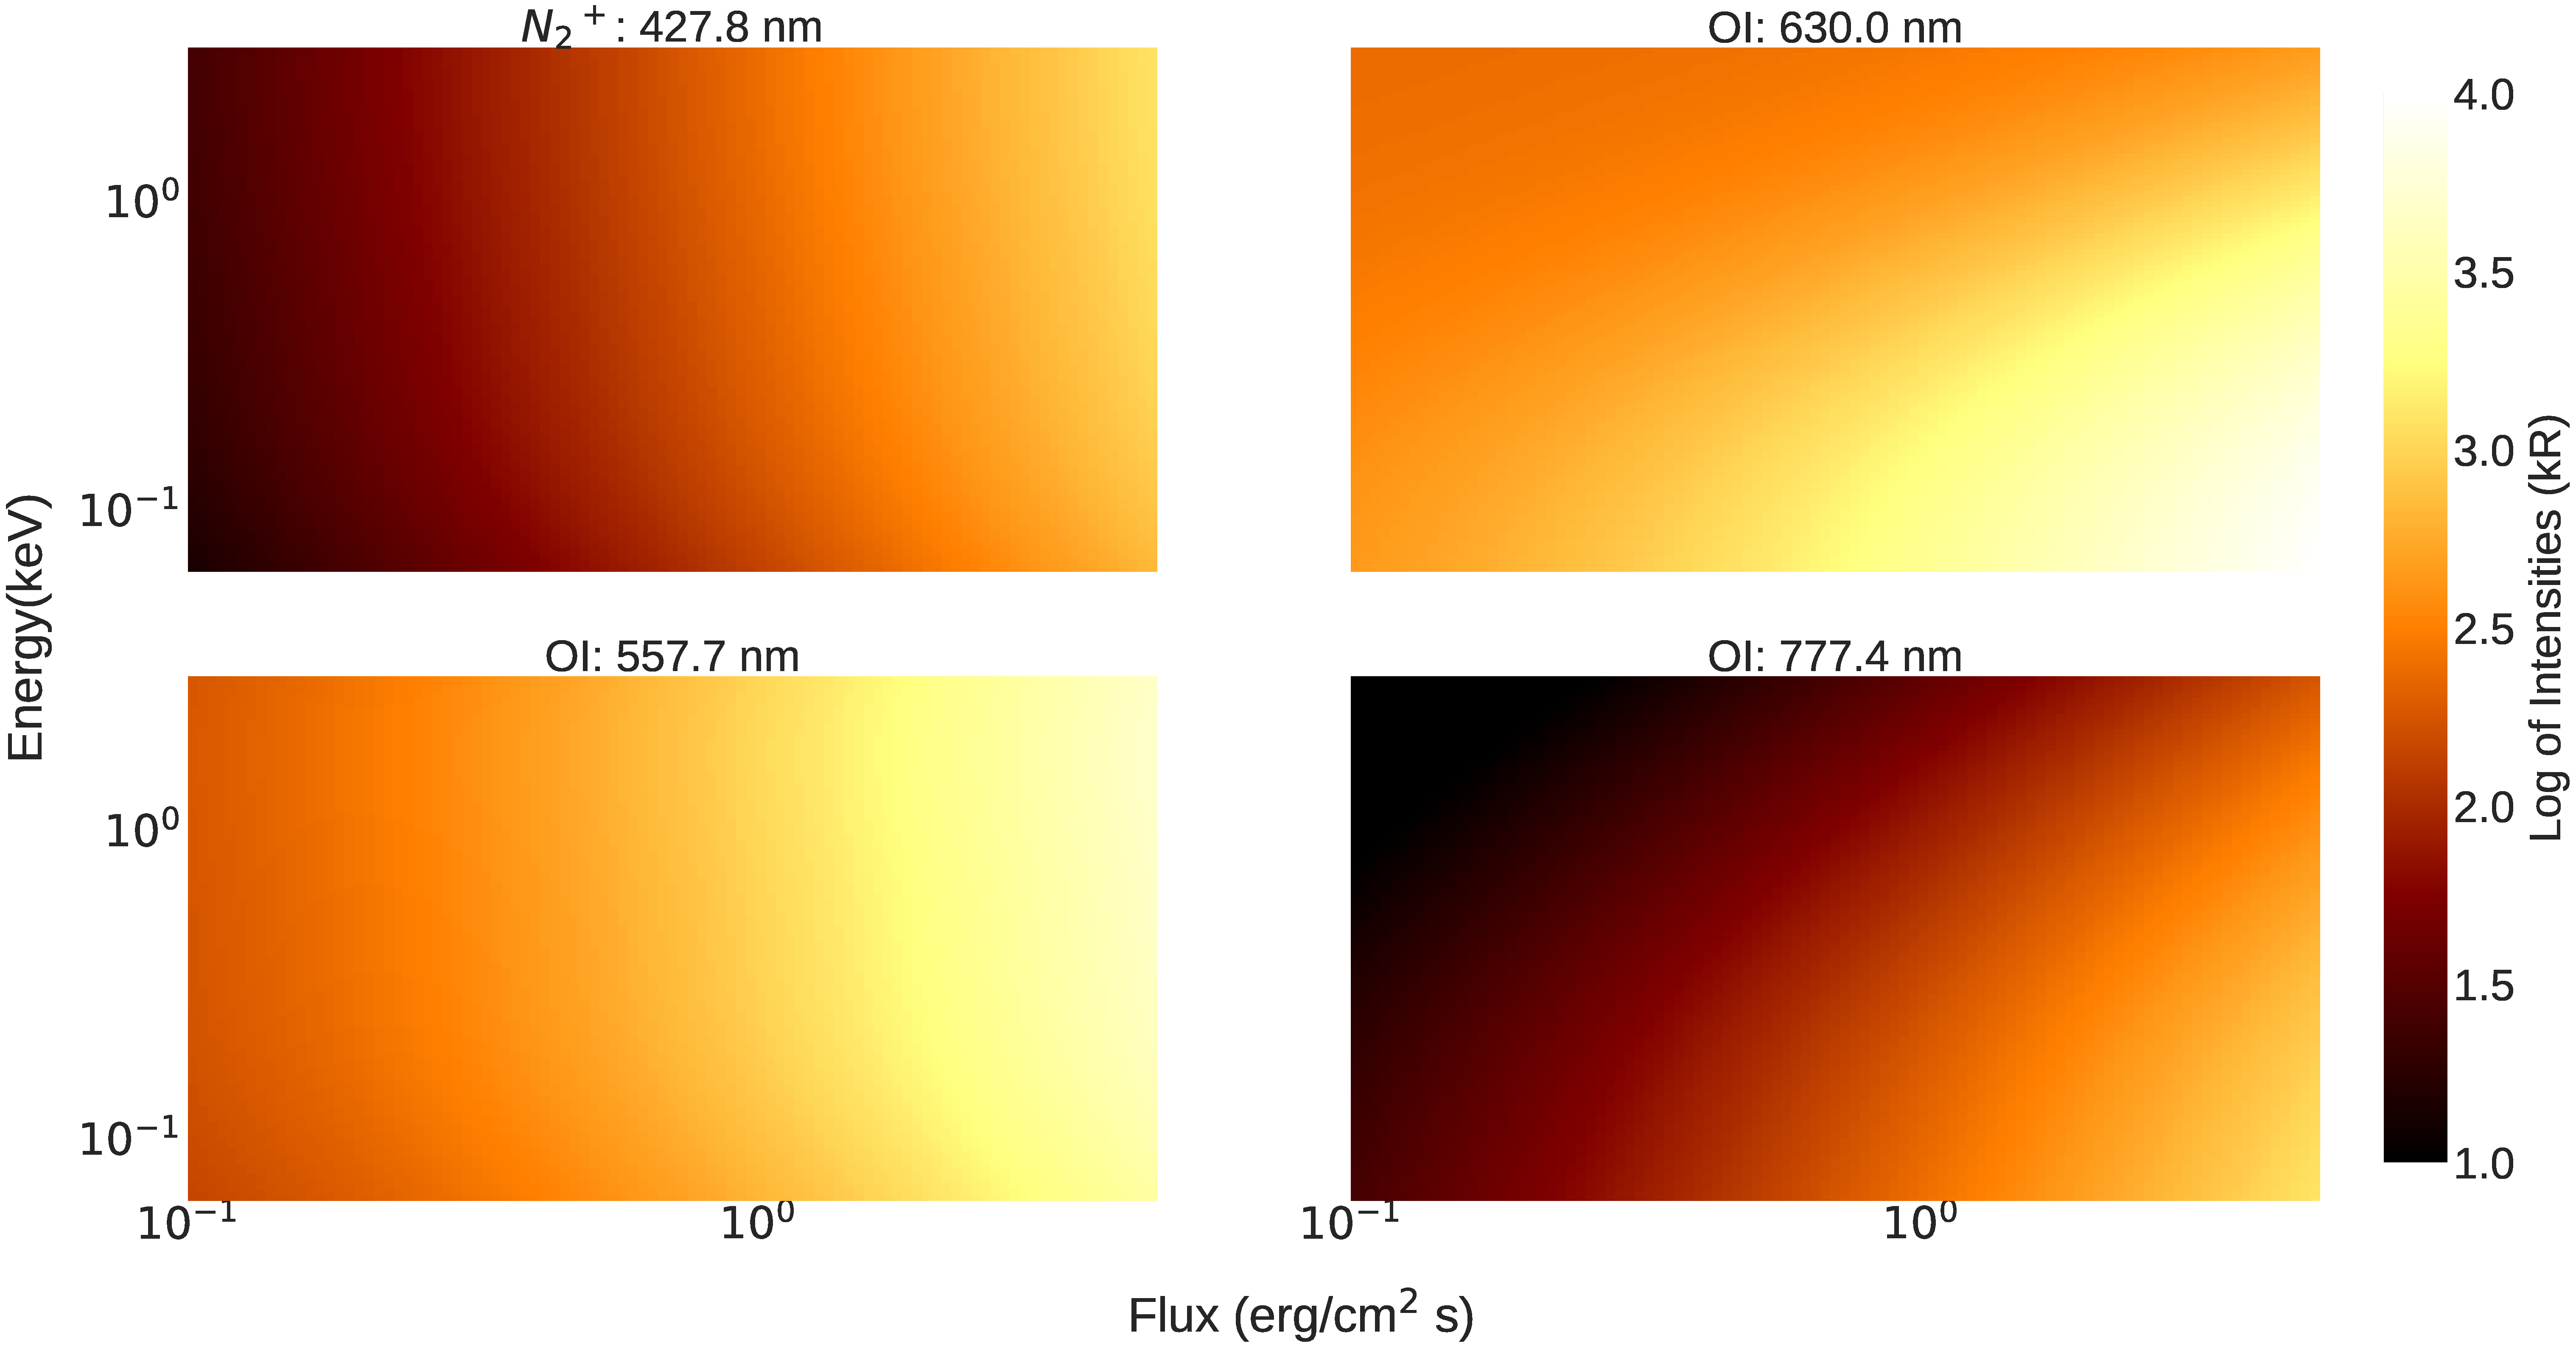
\includegraphics[width=30pc]{b_vs_e.pdf}
% \caption{Line of sight brightnesses as a function of characteristic energy and energy flux as predicted by GLOW at 9:50 PM on June 23 using IRI-90 and NRLMSIS00 ion and neutral parameters, respectively.}
% \label{fig:bve}
% \end{figure}
%\begin{figure}
% \centering\includegraphics[width=30pc]{b_e_f_r.eps}
% \caption{Brightness ratios as a function of energy and energy flux for the selected features}
% \label{fig:chi}
% \end{figure}
%%%%%%%%%%%%%%%%%%%%%%%%%%
\section{Energy and Flux derivation from optical emissions}
\subsection{Motivation for method selection}
The hmF2 is sensitive to changes in energy of the precipitating electrons because this determines where the electrons are stopped \citep{rees_1963}. \cite{pallamraju_2011} used this concept to derive the energy of precipitating electrons. Similarly, \cite{rees_1974} utilize red to blue line brightness ratios to infer the energy of the precipitating electrons. The red line emission peaks at higher altitudes and the blue line peaks at lower altitudes making them more sensitive to low and high energy electrons, respectively (Figure \ref{fig:vve}). Thus, their brightness ratio is sensitive to the energy of precipitating electrons. Also, as all the brightnesses increase with flux, \cite{pallamraju_2011} and \cite{rees_1963} use the red and the blue brightnesses, respectively, to estimate the flux. In addition, \citet{grubbs_compare} use the OI 844.6 to green line ratio and the blue line brightness in conjunction with a modified version of the GLOW model to derive energy and flux during an auroral event. Like the red line, the OI 844.6 nm emission peaks at higher altitude and is more sensitive to low energy electrons. \citet{grubbs_compare} compared the energy and flux derived using the optical method in situ particle measurements and found good correlation within 20$^\circ$ of magnetic zenith.

For our study, we explore whether or not the brightnesses or the brightness ratios of the three auroral features alone can be used to simultaneously derive both energy and fluxes. This was done by comparing the simultaneously derived energies and fluxes with a hybrid method using ratios to infer energy and then brightnesses to infer fluxes for comparison. 

\subsection{Methods}
We compare three different methods, summarized in Table \ref{table:method}, to derive electron energies and fluxes for the June 22-23, 2015 aurora. 
All of the methods were based on the iterative non-linear minimization of chi-square ($\chi^2$, weighted least-squares) at each observation time, t:


\begin{equation}
\chi^{2}_t (E,Q) = \sum_{i}\Bigg({\frac{O_{i} - M_{i} (E,Q)} {\sigma_{i}}}\Bigg)^{2}.
% +({\frac{O_{557} - M_{557}} {\sigma_{557}}})^2+({\frac{O_{427} - M_{427}} {\sigma_{427}}})^2+({\frac{O_{777} - M_{777}} {\sigma_{777}}})^2
\label{eq:chi}
\end{equation}
Here, at time t, $O_{i}$ and $M_{i}$ are the observed and modeled brightnesses (or brightness ratios) of $ i^{th}$ emission feature, respectively, and $\sigma_{i}$ represents the standard deviation (in brightness) of the $ i^{th}$ emission feature. Energy ($E$) and flux ($Q$) are input into the GLOW model and are iteratively varied to minimize $\chi^2$ (Equation \ref{eq:chi}) using the Levenberg-Marquardt algorithm (LMA) \citep{levenberg,marquardt}. LMA is based on a combination of gradient descent (towards minimum) and residual (in our case $\chi^2$, the weighted squared residual) minimization methods. The covariance matrix returned by this method gives us the statistical uncertainties in the derived parameters which were taken to be the final uncertainties since the model uncertainties are not considered. 

We applied the three methods mentioned below to derive energy and flux (summarized in Table \ref{table:method}) by performing the non-linear minimizations using the $LMFIT$ module for Python \citep{lmfit}. For our results, we report the characteristic energy of the Maxwellian distribution, $E_0$, as discussed in section \ref{sec:model}. For a Maxwellian distribution, to convert to average energy ($E_{av}$), $E_0$ can be multiplied by a scaling factor, i.e., $E_{av}$ = 2 $E_0$ \citep{kosch_2001}.
\subsubsection{Brightness method}
\label{sec:brightness}
In this method, the modeled brightnesses in red, green and blue lines were compared with the measurements by simultaneously varying $E$ and $Q$ inputs into the GLOW model to minimize $\rm \chi^2$. This method explores the feasibility of directly comparing model with the measurements to derive energies and fluxes of auroral electron precipitation.

\subsubsection{Ratio method}
\label{sec:ratio}
In this method, the modeled ratios of blue to red, blue to green and green to red lines were compared with the measured ratios to derive energies and fluxes of precipitating electrons. This was done in similar fashion as the brightness method (section \ref{sec:brightness}) by varying $E$ and $Q$ simultaneously to minimize $\rm \chi^2$. 

\subsubsection{Hybrid method}
\label{sec:2step}
%This method is similar to that used by \cite{pallamraju_2011} where energies and fluxes were derived using two steps. \cite{pallamraju_2011} first estimated energies using simultaneous HmF2 measurement by a nearby ISR based on the formalism of
%\cite{rees_1963}. Then, the energy fluxes were estimated by varying flux input to the GLOW model until the model matched the measured red line brightness at the derived energy.

\cite{pallamraju_2011} had only the red line brightness measurements and so used the electron density profile ($N_e$) from ISR measurements to derive energies of the precipitating electrons. GLOW model red line brightness (at the derived energies) were then constrained with measurements to derive energy fluxes. Since we have simultaneous measurements of three emission features, we used the brightness ratios to predict the energies following a method similar to \cite{rees_1974} and then used the brightnesses to derive fluxes. First, the modeled brightness ratios of the blue to red, blue to green and red to green lines were compared with the measured brightness ratios to derive energies. This was done by varying $E$ to minimize $\rm \chi^2$ while $Q$ was kept constant at 1 erg $\rm cm^{-2} s^{-1}$. Then, at the derived energy ($E_0$), $Q$ was varied in the GLOW model to minimize $\rm \chi^2$ to compare the model brightnesses of red and green lines with the measured brightnesses. 


\begin{sidewaystable}
	
	\caption{Summary of the three different methods used to minimize $\chi^2$ in Equation \ref{eq:chi}.}
	\begin{tabular}{|l|l|}
		\hline
		
		Method &  Approach \\
		\hline
		\centering
		Brightness & \makecell{Constrain $E$ and $Q$ simultaneously\\ by comparing model brightness with measurements}\\ 
		
		\hline
		Ratio  &  \makecell{Constrain $E$ and $Q$ simultaneously\\ by comparing modeled brightness ratios with measurements}\\
		\hline
		
		Hybrid & \makecell{Step 1: Keep $Q$ constant and constrain $E$\\
			by comparing model brightness ratios with measurements\\
			\hline			
			Step 2: At $E$ derived in Step 1, constrain $Q$\\
			by comparing model brightness with measurements}\\
		\hline
	\end{tabular}
	\label{table:method}
\end{sidewaystable}
\section{Results}
Figure \ref{fig:e_fl_3mtd} shows the results derived using these methods for one selected look direction (37-54$^\circ$ ZA). The results are similar for other look directions. The hybrid method produced the least uncertainties in the derived energies and fluxes given by the minimization routine (Figure \ref{fig:e_fl_3mtd}). However, for flux derivation the uncertainties in the derived energies cannot be propagated without modifying the GLOW model. Using the upper and lower energy limits of the derived energy as input into the GLOW model, the difference in derived fluxes, assumed to be the estimated uncertainty in fluxes due to the uncertainty in energies, were found to be insignificant (in the range of $\approx$ $\pm$0.01 erg $\rm cm^{-2} s^{-1}$). Also, as mentioned in section \ref{sec:2step}, the hybrid method uses a constant flux input into the GLOW model during the first step to derive energies. We varied the initial flux estimates from
0.1 erg $\rm cm^{-2} s^{-1}$ to 50 erg $\rm cm^{-2} s^{-1}$ and found that the derived results did not vary significantly for flux values greater than 0.1 erg $\rm cm^{-2} s^{-1}$ (Figure \ref{fig:fl_d}). The derived energies for this method ranged from 57 eV to 278 eV while the flux ranged from 0.8 to 2.8 erg $\rm cm^{-2} s^{-1}$ 
%  This method also produced the best match between the measured red and green line brightnesses and the model estimates with the derived energies and fluxes as inputs into GLOW (Figure \ref{fig:e_fl_b_comp}).

% The brightness method was initially applied by using all four emission brightnesses. Using the additional OI (777.4 nm) line, however, increased the uncertainties in the derived quantities. Using the red, green and blue lines, the energies and fluxes derived using the brightness method were similar to the hybrid method. 

% This method also produced good match with the measured red and the green line brightnesses when the derived energies and fluxes were set as inputs back into the GLOW model (Figure \ref{fig:e_fl_b_comp}). 

The ratio method had the highest uncertainties in the derived energy and fluxes (Figure \ref{fig:e_fl_3mtd}). The energies and fluxes derived using this method were also not in agreement with the brightness and the hybrid methods. The derived energies for the ratio method ranged from 52 eV to 1200 eV while the flux ranged from 0.08 to 10 erg $\rm cm^{-2} s^{-1}$ 

% In addition, the retrieval of the red and the green line profile with the derived energies and fluxes as input was not accurate (Figure \ref{fig:e_fl_b_comp}). 
% 
%The hybrid method produced the best results but needed a flux to be picked in the first step and the errors in the energy derived in the first step was not propagated to the second step. 
%To study why the ratio method differed significantly from the other two methods, we plotted the $\rm \chi^2$-values at two times with different results (00:08 and 01:27 LT on June 23,2015) as a function of characteristic energy and total energy flux using for the two simultaneous minimization methods (brightness and the ratio methods in Figure \ref{fig:chi_08} and Figure \ref{fig:chi_127}, respectively). At 00:08, the derived energies and fluxes using the ratio method are very different from the hybrid and brightness methods while, at 01:27 the derived energies using all three methods are similar. Figures \ref{fig:chi_08} and \ref{fig:chi_127} show that while the brightness method is sensitive to both energy and flux, the ratio method is only sensitive to the energy. We speculate that because all the brightnesses increase with increasing flux, we lose the flux information when we take the brightness ratios. In addition, for the brightness method, the $\rm \chi^2$-values rise quickly away from the minimum (tightly constrained minimum $\rm \chi^2$). However, for the ratio method, there is a spread of similar values even far away from the minimum which makes the minimization more susceptible to systematic errors, including those caused by our viewing geometry. At 00:08 LT (T3 in Figure \ref{feature:nbrg}), we saw brightness changes with look direction (brighter farther north) in the red line emission which is visible from farther north compared to blue and green line (Figure \ref{fig:elayer}). The changes in the blue and green line brightnesses with zenith angle at the same time were minimal. Thus, we could have been looking at different aurora farther north (in red line) at this time. This should also affect the hybrid and the brightness method, and we see there is larger mismatch between the retrieved blue line brightness at 00:08 LT using the hybrid and the  brightness methods compared to 1:27 AM (Figure \ref{fig:e_fl_b_comp}). Furthermore, the lack of sensitivity to average flux could also cause the energies to be derived incorrectly because the minimization of $\rm \chi^2$ using the ratio method depends both on energy and flux parameters simultaneously.

To study why the results obtained from the ratio method differed so significantly from the results of the other two methods, we plotted the $\rm \chi^2$-values from 00:08 and 01:27 LT on June 23, 2015, as a function of characteristic energy and total energy flux. Results from the brightness and ratio methods are shown in Figures \ref{fig:chi_08} and \ref{fig:chi_127} respectively. At 00:08, the energies and fluxes derived using the ratio method are very different from those given by the hybrid and brightness methods, while at 01:27 the energies derived using all three methods are similar. Figures \ref{fig:chi_08} and \ref{fig:chi_127} show that while the brightness method is sensitive to both energy and flux, the ratio method only appears to be sensitive to variations in energy. We speculate that this is because the flux information is lost when the brightness ratios are determined, since all the brightnesses increase with increasing flux. In addition, Figure \ref{fig:chi_08} shows a tightly constrained minimum $\rm \chi^2$ for the brightness method, away from which the $\rm \chi^2$ values rise quickly. However, for the ratio method, shown in Figure \ref{fig:chi_127}, similar $\rm \chi^2$ values are found far away from the minimum, suggesting that the minimization will be more susceptible to systematic errors, including those caused by our viewing geometry. At 00:08 LT (T3 in Figure \ref{feature:nbrg}), we saw an increase in brightness toward the north in the red line emission, while the changes in the blue and green line brightnesses with zenith angle were minimal. Because the red line aurora is visible from farther north compared to blue and green line emissions (Figure \ref{fig:elayer}), it is possible that we could have been looking at spatially separated features in the red line aurora, which were unrelated to the blue and green line emissions at the same time. If this were true, it would also affect the accuracies of the hybrid and the brightness methods. Indeed, we see that there is larger mismatch between the retrieved blue line brightness at 00:08 LT using the hybrid and the brightness methods compared to 01:27 LT (Figure \ref{fig:e_fl_b_comp}). Furthermore, the lack of sensitivity to average flux could also cause the energies to be derived incorrectly, since the minimization of $\rm \chi^2$ using the ratio method depends on both the energy and flux parameters simultaneously.

The hybrid method also uses the brightness ratio in the first step; however, for a fixed flux (1 erg $\rm cm^{-2}s^{-1}$), $\rm \chi^2$ (using brightness ratio) is sensitive to energy (Figure \ref{fig:chi_hybrid}). In the second step, at the energy derived in step one, we minimized $\rm \chi^2$ using brightness to derive fluxes as brightnesses are sensitive to changes in flux.

The brightness method produced results similar to the hybrid method without requiring an initial guess of $Q_0$. Additionally, the computational time for the brightness method was around 33\% faster using a single core CPU (for 249 data points) compared to the hybrid method. The retrieval of red and green line brightnesses from both hybrid and brightness methods, by using the derived energies and fluxes as inputs to GLOW model, were consistent with the observed brightnesses. The temporal morphology of blue line brightnesses were reconstructed correctly but the brightness values were overestimated (Figure \ref{fig:e_fl_b_comp}). This could be because the MSIS neutral densities are not accurate during storm time \citep{fang_variations_2012}. Furthermore, since all of our measurements are off-zenith, we could be measuring auroras from different locations especially for higher zenith angles (this is true for all three methods).

Results derived using the ratio method, on the other hand, were not in good agreement with the other two methods (Figure \ref{fig:e_fl_3mtd}). Furthermore, the brightnesses retrieved using the ratio method did not match the observed brightness (see Figure \ref{fig:e_fl_b_comp}). We thus conclude that the ratio method may not be a suitable method to derive energies and fluxes during an aurora. Since the hybrid and the brightness methods produce very similar results, only the results derived using the brightness method are shown for the remainder of this paper.

The temporally averaged energies and fluxes derived using the brightness method are summarized in Table \ref{table:efl_look}. These results were obtained by deriving energy and flux at each observation time and then averaging over each of the selected time intervals T1 to T8 (shown in Figure \ref{feature:nbrg}). The energy values derived ranged between 109 to 262 eV while the flux values ranged from 0.8 to 2.2 erg $\rm cm^{-2} s^{-1}$.


\subsection{Energy and Flux Morphology}
\label{sec:emorph}
The derived energies and fluxes show both temporal and spatial variations, as seen in Figure \ref{fig:e_fl_la}. The derived energies were lower and the fluxes higher for small zenith angles during most of time period T1. Temporally, there was a sharp drop in energy and increase in flux during this period, especially at 20-37$^\circ$ ZA. These are consistent with red line brightness profile during the period T1 (Figure \ref{feature:nbrg}) where the brightness was higher for small zenith angles and there was a sudden rise in brightness temporally.
%since the red line is more sensitive to lower energies as the emission originates at higher altitudes. %Hence, for time period T1, the red line brightness was also decreasing for higher zenith angles.

Spatially, for most of time periods T3, T4 and T8 the conditions were opposite (compared to the period T1) with higher energies and lower flux at smaller zenith angles. This is consistent with the increase in the red line brightnesses for higher zenith angle during these periods. As discussed in section \ref{sec:bmorph}, for these periods (T3, T4 and T8), the brightness increase in red line for higher zenith angles was sharp but there were no significant brightness changes in other features. The red line emission is visible farther north (and is always north for a given look direction) because of HiT\&MIS's orientation and the emission's occurrence at a higher altitude compared to the other two lines (Figure \ref{fig:elayer}). So, we could be detecting auroral structure only visible in red line. Hence, the derived energies and fluxes for these time periods should be treated with caution. Also, since the red line covers a larger latitudinal range, we might be observing a gradient in brightness that was not as apparent in blue and green line brightnesses. 

In addition, SAR (Stable Auroral Red) arcs, that are common in the mid-latitude during geomagnetic storms \citep{mendillo_sar}, can cause brightness enhancements only in the red line. The production source of SAR arcs are thermal fluxes from the inner magnetosphere and not electron precipitation (see \cite{mendillo_sar}; \cite{kozyra_1997,rees_1975} and references therein). Boston University (BU) all-sky images (\cite{asi_1993}) from Millstone Hill (approximately 10 miles southwest of Lowell, MA) show SAR arc in red line data towards the south and not close to HiT\&MIS's FOV (Figure \ref{fig:allsky}). SAR arcs can occur along with aurora near the equatorial edge of aurora \citep{ievenko_2008}; however; we do not see any evidence of this by examining all available BU red line all-sky image data during our observation period. Nonetheless, there were time periods when the sky was cloudy over Millstone Hill but clear in the HiT\&MIS FOV. Thus, we do not completely rule out the possibility of SAR arcs being present in our FOV at those times. This could result in derived energies that are lower than the true energies and the fluxes to be higher than the true fluxes. 

In the time period T2, the increase in the derived energy corresponds to the peaks in the blue line profiles. The fluxes during most of the time period T2 remained relatively constant indicating that the brightness variations were due to increase in the energy of precipitating electrons. The decrease in energy towards the end of the time period T2 was due to the increase in the red line brightness indicating more electrons (higher flux) with slightly less energy precipitated. 

The derived energies are increasing with time during the period T5 while the fluxes are slightly decreasing. The blue and green line brightnesses during the same time period were increasing similarly to the derived energies while the red line brightness was slowly decreasing. Since the green and blue line emissions occur at much lower altitudes (approximately 150 km and 100 km, respectively) than the red line, they are sensitive to higher energy electrons. This indicates that the energies of the precipitating electrons increased with time during the time period T5 causing the blue and green lines to get brighter, despite the slight decrease in flux.

During the time period T6, all the emission brightnesses increased, with the increase in the red line being most prominent than other features. The derived energies show a decreasing trend with time. Since red line brightness is more prominent for lower energies, it makes sense that T6 shows enhanced red line brightness. Due to an increase in flux, the blue and the green lines also increased in brightness. Thus, the temporal and spatial morphologies in derived energies and fluxes are consistent with the brightness morphologies in Figure \ref{feature:nbrg}. 




%Derived energies and fluxes (at 37 to 54$^\circ$ zenith angle) using the brightness and the ratio methods were in good agreement with each other within the margin of 1-$\sigma$ uncertainty as seen in Figure \ref{fig:e_fl_3mtd}. The simultaneous ratio method on the other hand, was not in good agreement with the other methods for most time ranges. We inputed these derived energies and fluxes into the GLOW model to compute brightnesses and compare them with the brightness measurements as shown in Figure \ref{fig:e_fl_b_comp}. Again for the brightness and the ratio methods, the retrieved profile showed excellent agreement with the original brightness profiles for the red and the green lines, and fair agreement with the blue line. However, the profiles retrieved using the simultaneous ratio method was not in good agreement with the original profiles. We thus concluded that the simultaneous ratio method, where derivation were done by minimizing brightness ratios using two parameter variation in energy and flux parameters, was not a suitable method to derive energies and fluxes.






\begin{figure}
	\centering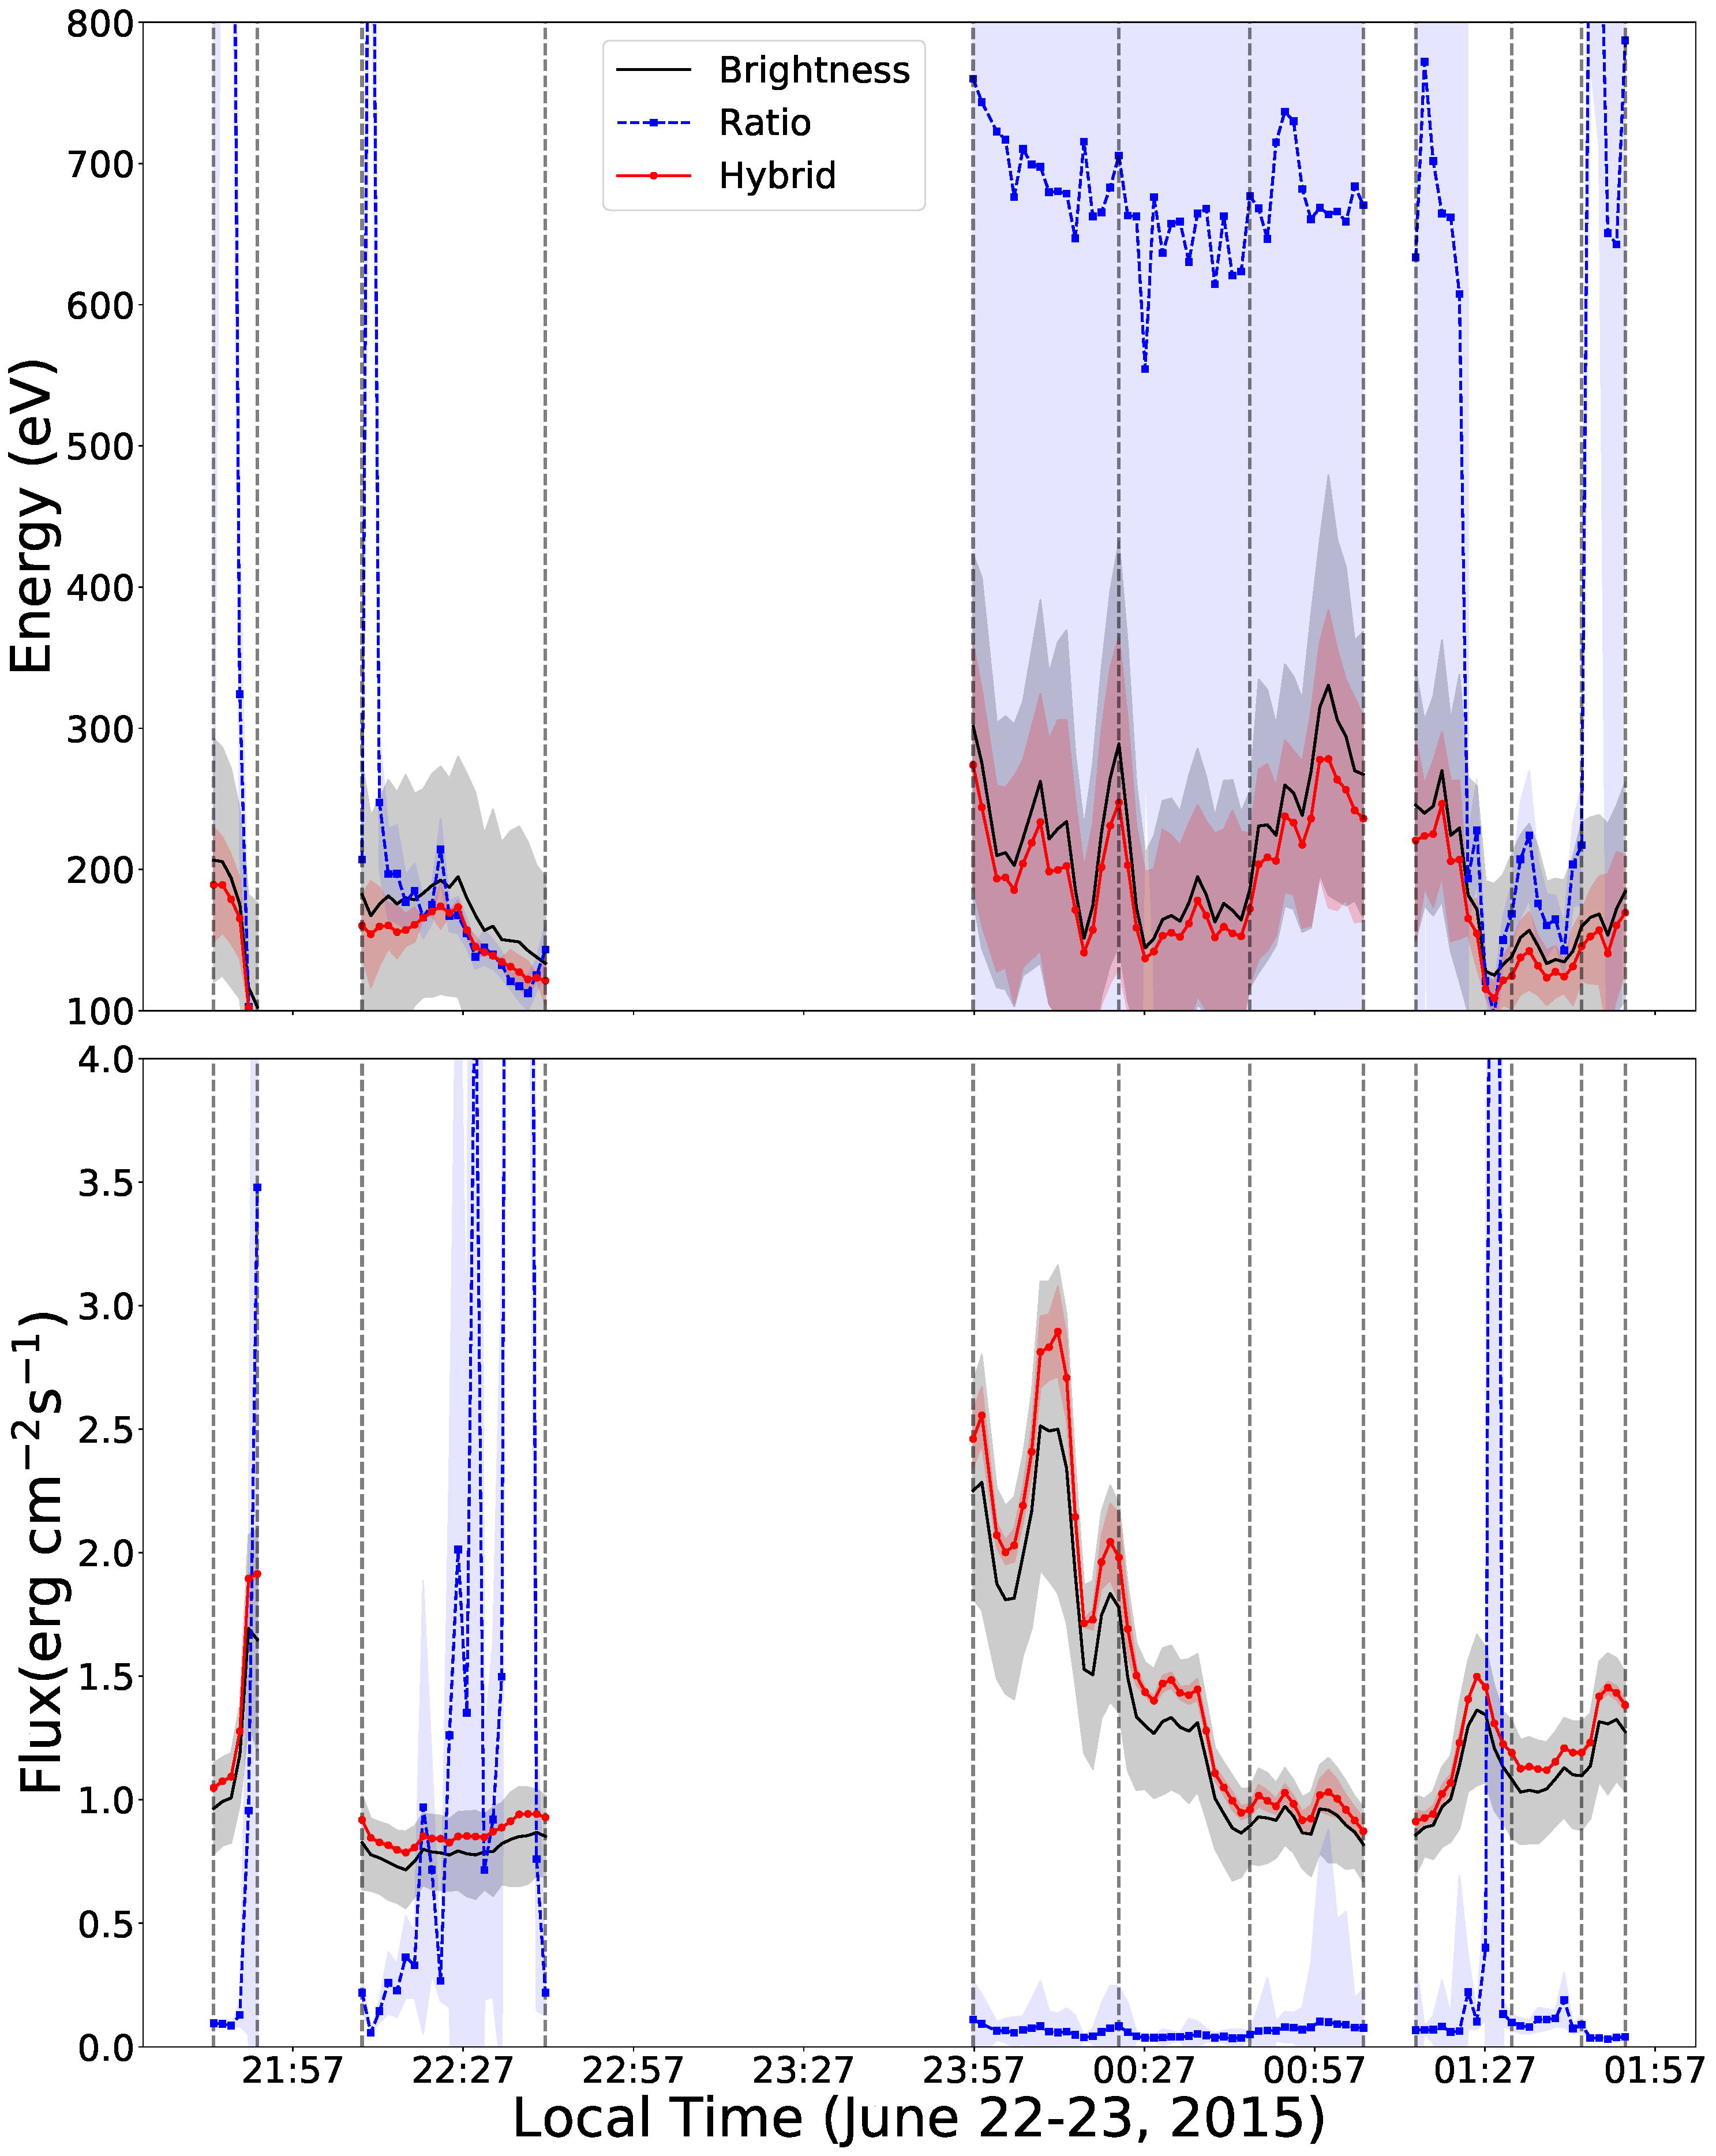
\includegraphics[width=30pc]{different_method_e_fl.pdf}
	\caption{Energies and fluxes derived from 37 to 54$^\circ$ ZA by using three different methods on June 22-23, 2015. Shaded regions denote $\pm$ 1-$\sigma$ statistical uncertainty in the derived results. The brightness and the hybrid methods are in good agreement with each other while for the ratio method, the derived energies and fluxes are inconsistent with the other two methods and the derived uncertainties are significantly larger. Blank areas denote cloudy times based on the NeI 630.5 nm line shown in Figure \ref{feature:nbrg}.}
	\label{fig:e_fl_3mtd}
\end{figure}
\begin{figure}
	\centering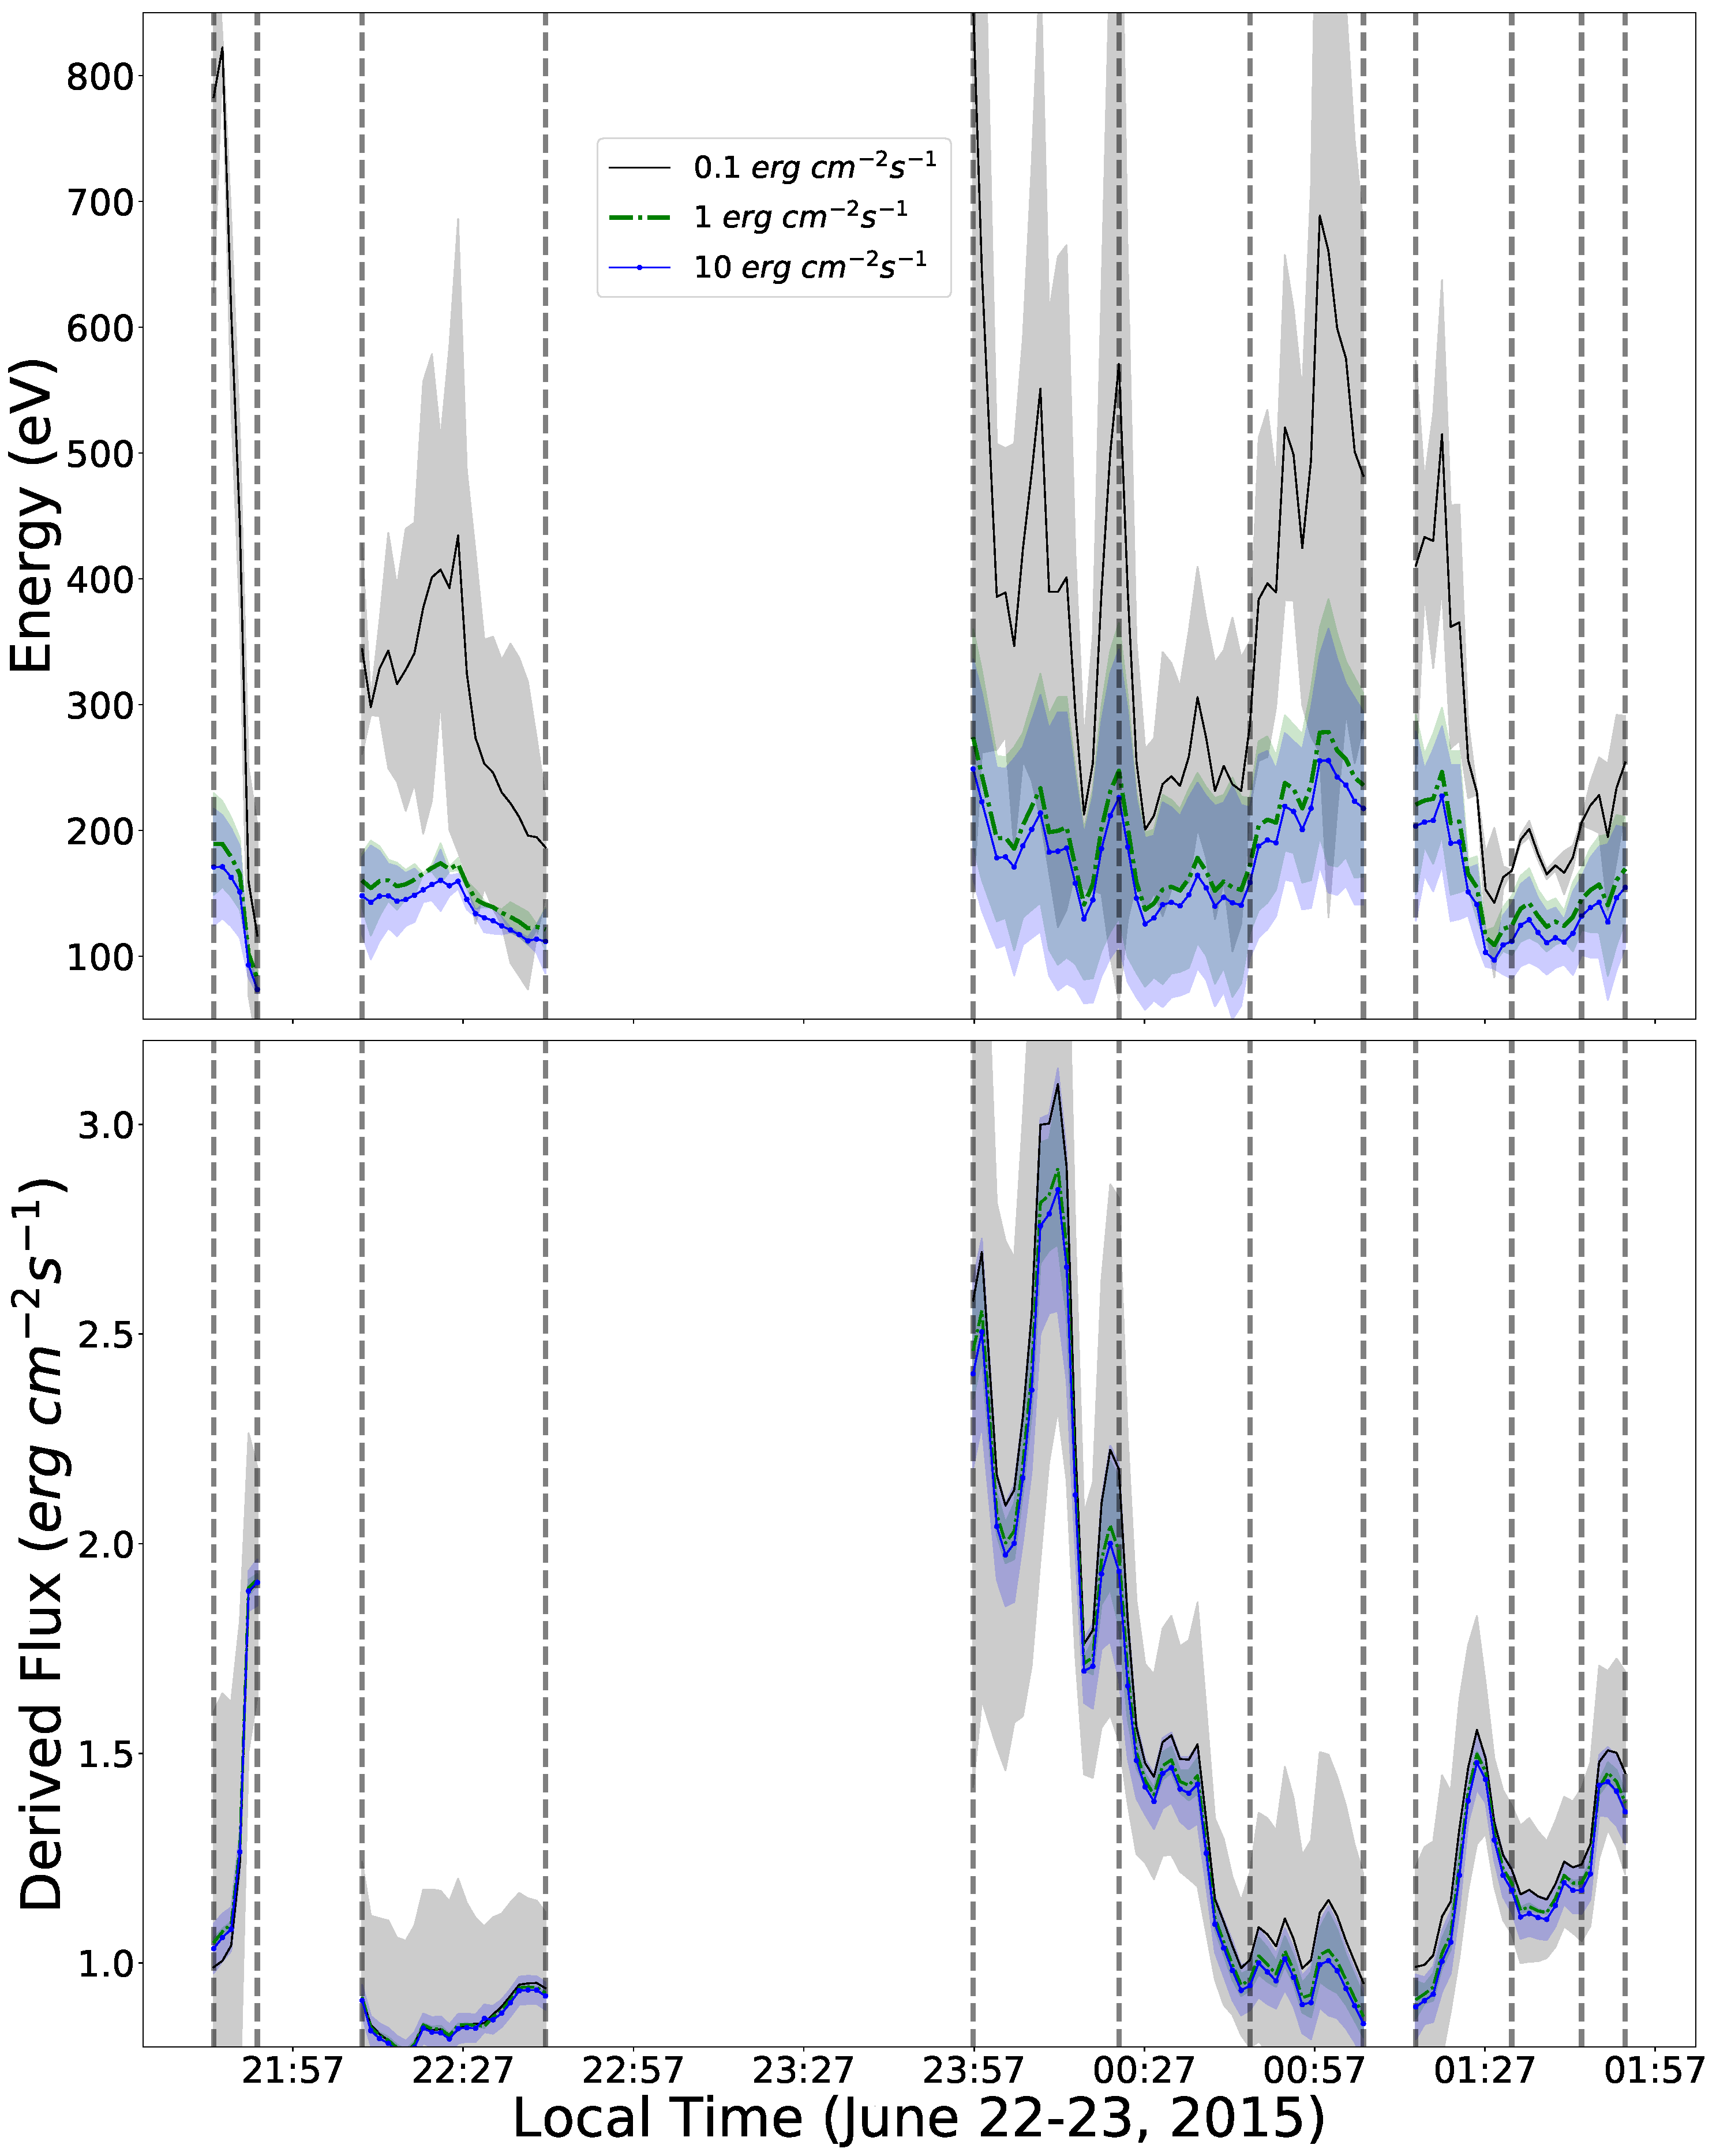
\includegraphics[width=30pc]{ratio_method_dfl.pdf}
	\caption{Energies and fluxes derived from 37 to 54$^\circ$ ZA by using different initial input fluxes in the first step using the hybrid methods on June 22-23, 2015. Shaded regions denote $\pm$ 1-$\sigma$ statistical uncertainty in the derived results. Notice that derived energies and fluxes all match well except for the flux of 0.1 erg $\rm cm^{-2} s^{-1}$. Blank areas denote cloudy times based on the NeI 630.5 nm line shown in Figure \ref{feature:nbrg}.}
	\label{fig:fl_d}
\end{figure}
\begin{figure}
	\centering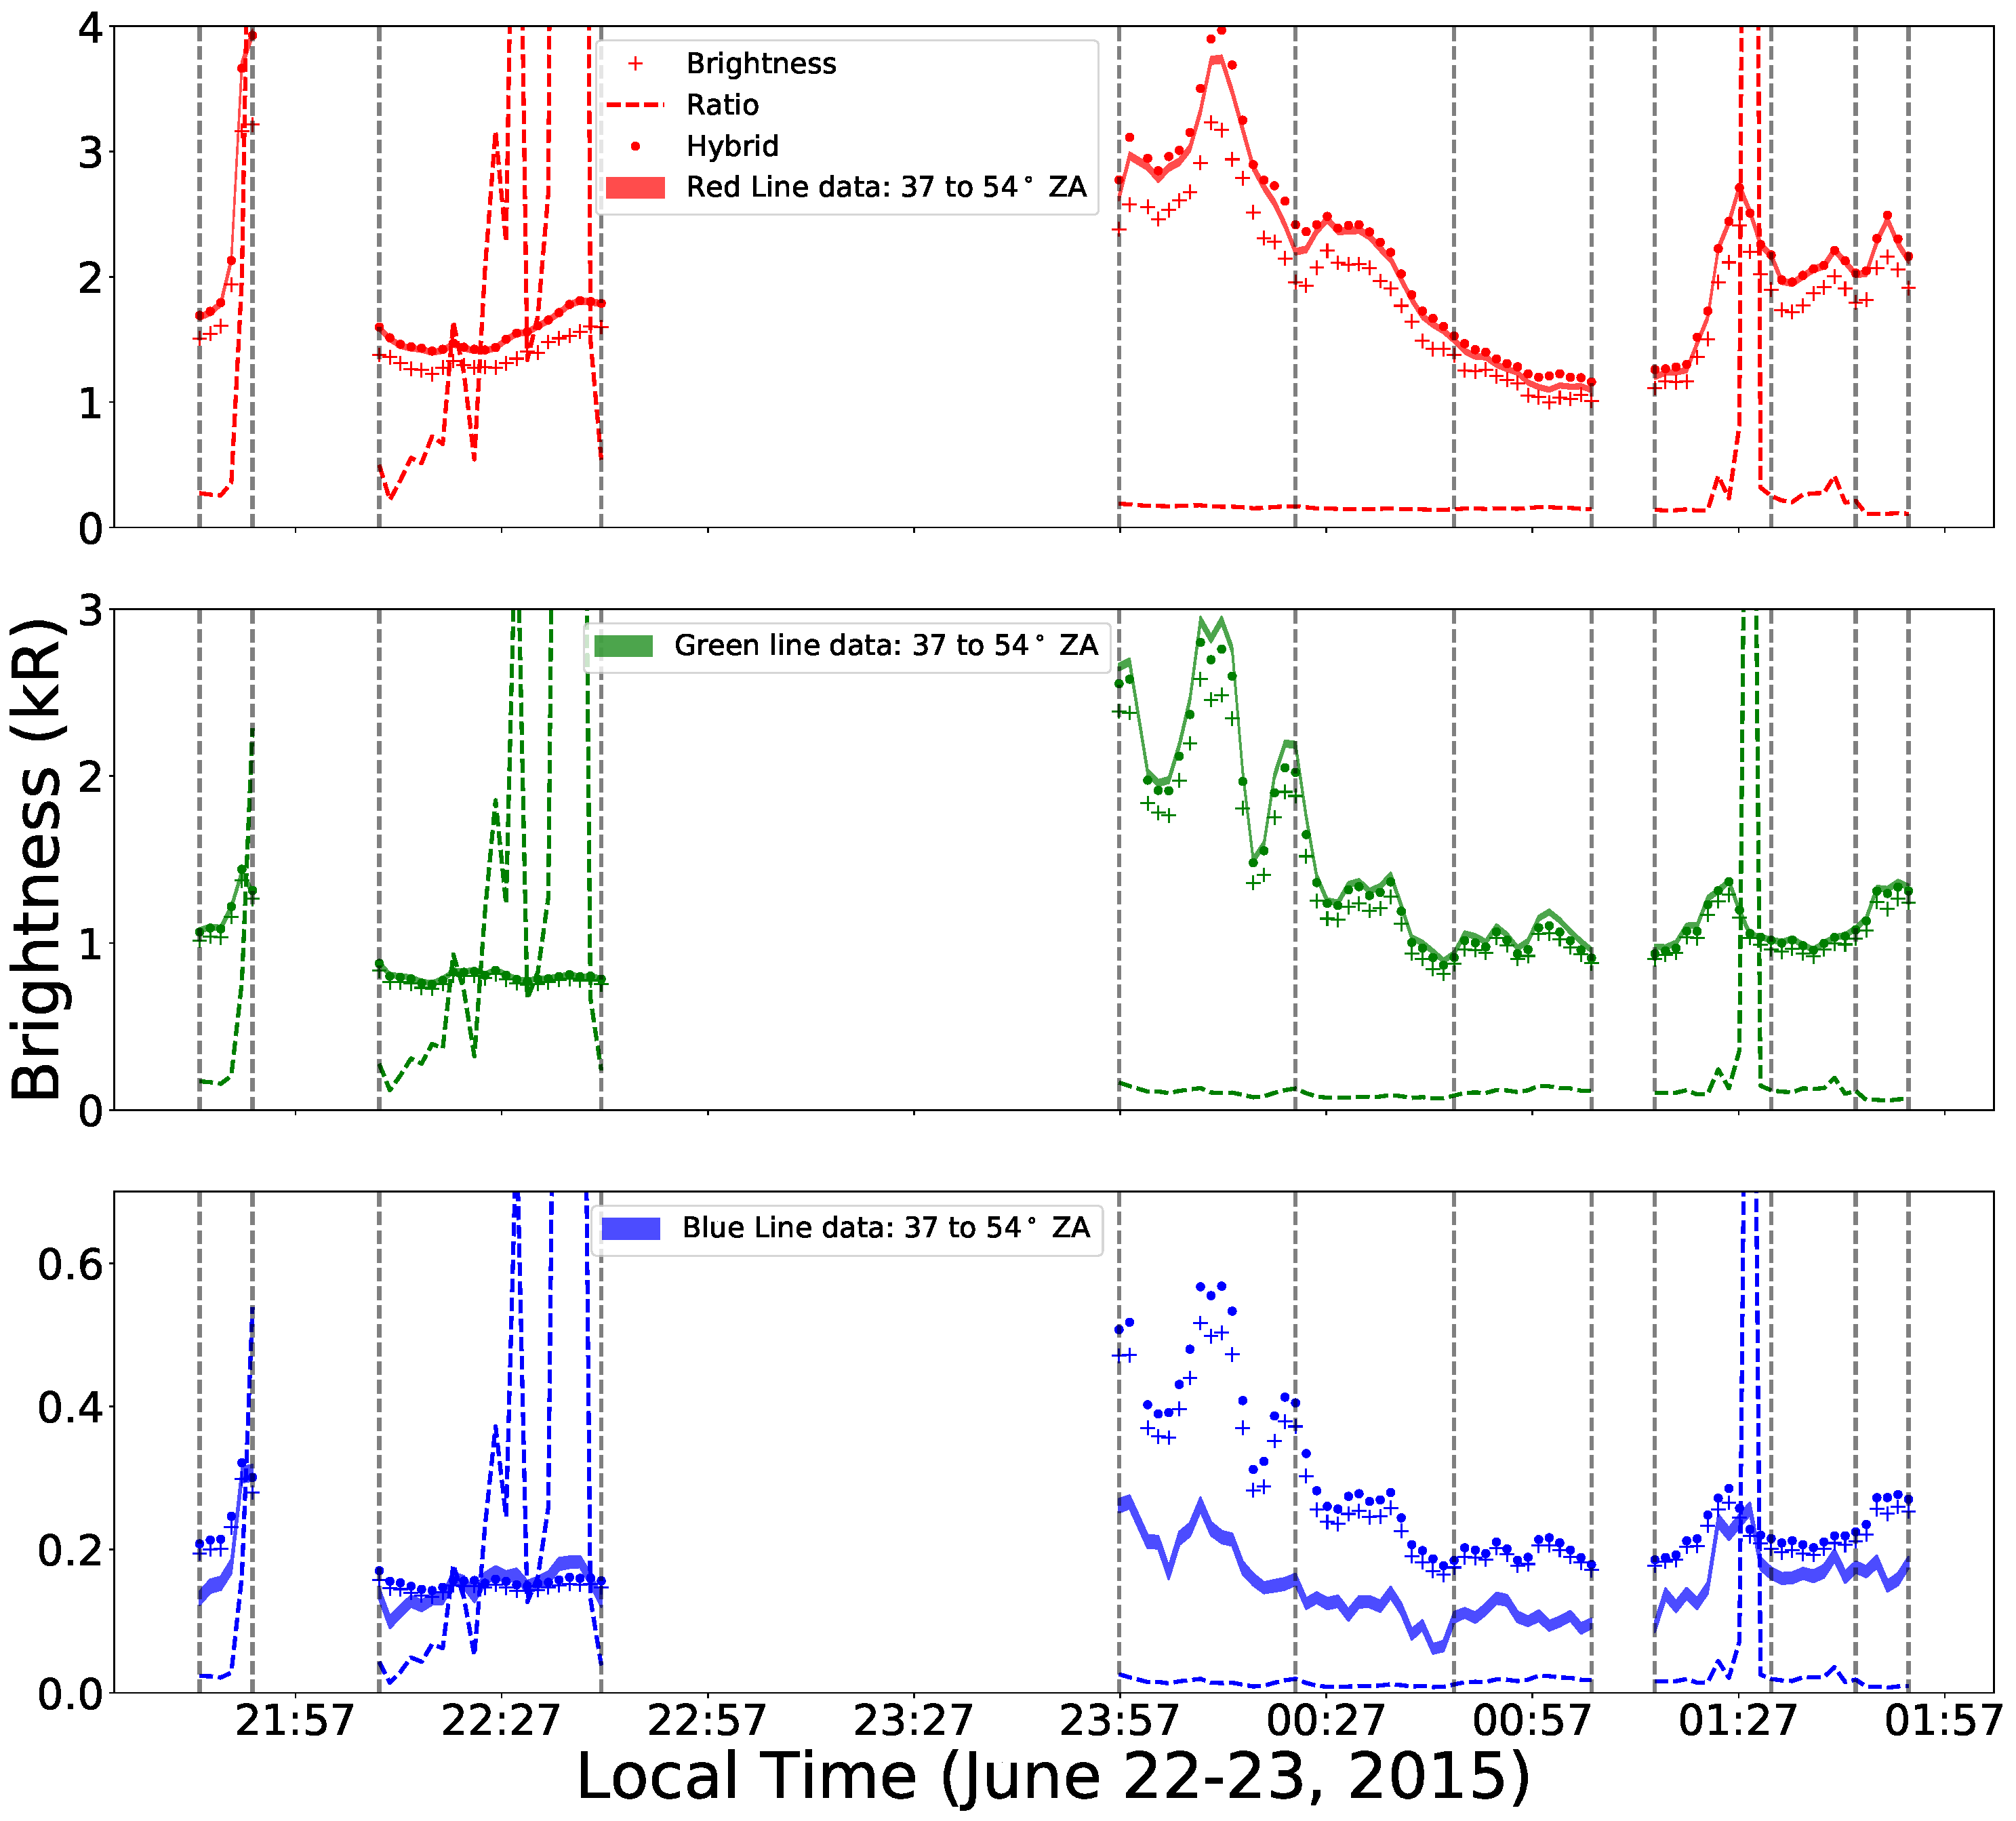
\includegraphics[width=35pc]{different_method_retriv_comp.pdf}
	\caption{Brightnesses retrieved from 37 to 54$^\circ$ ZA by using the derived energies and fluxes as inputs into the GLOW model are compared against measurements. The three different methods are shown with stars (brightness), dot (hybrid), and dashed (ratio) markers. The shaded regions denote the measured brightnesses within the $\pm$ 1-$\sigma$ uncertainty in the measurements which is more noticeable in the blue line data. Notice that the retrieved red and green brightnesses have a good match well with measured red, green line brightnesses for hybrid and the brightness methods but not for the ratio method. Blank areas denote cloudy times based on the NeI 630.5 nm line shown in Figure \ref{feature:nbrg}.}
	\label{fig:e_fl_b_comp}
\end{figure}
\begin{figure}
	\centering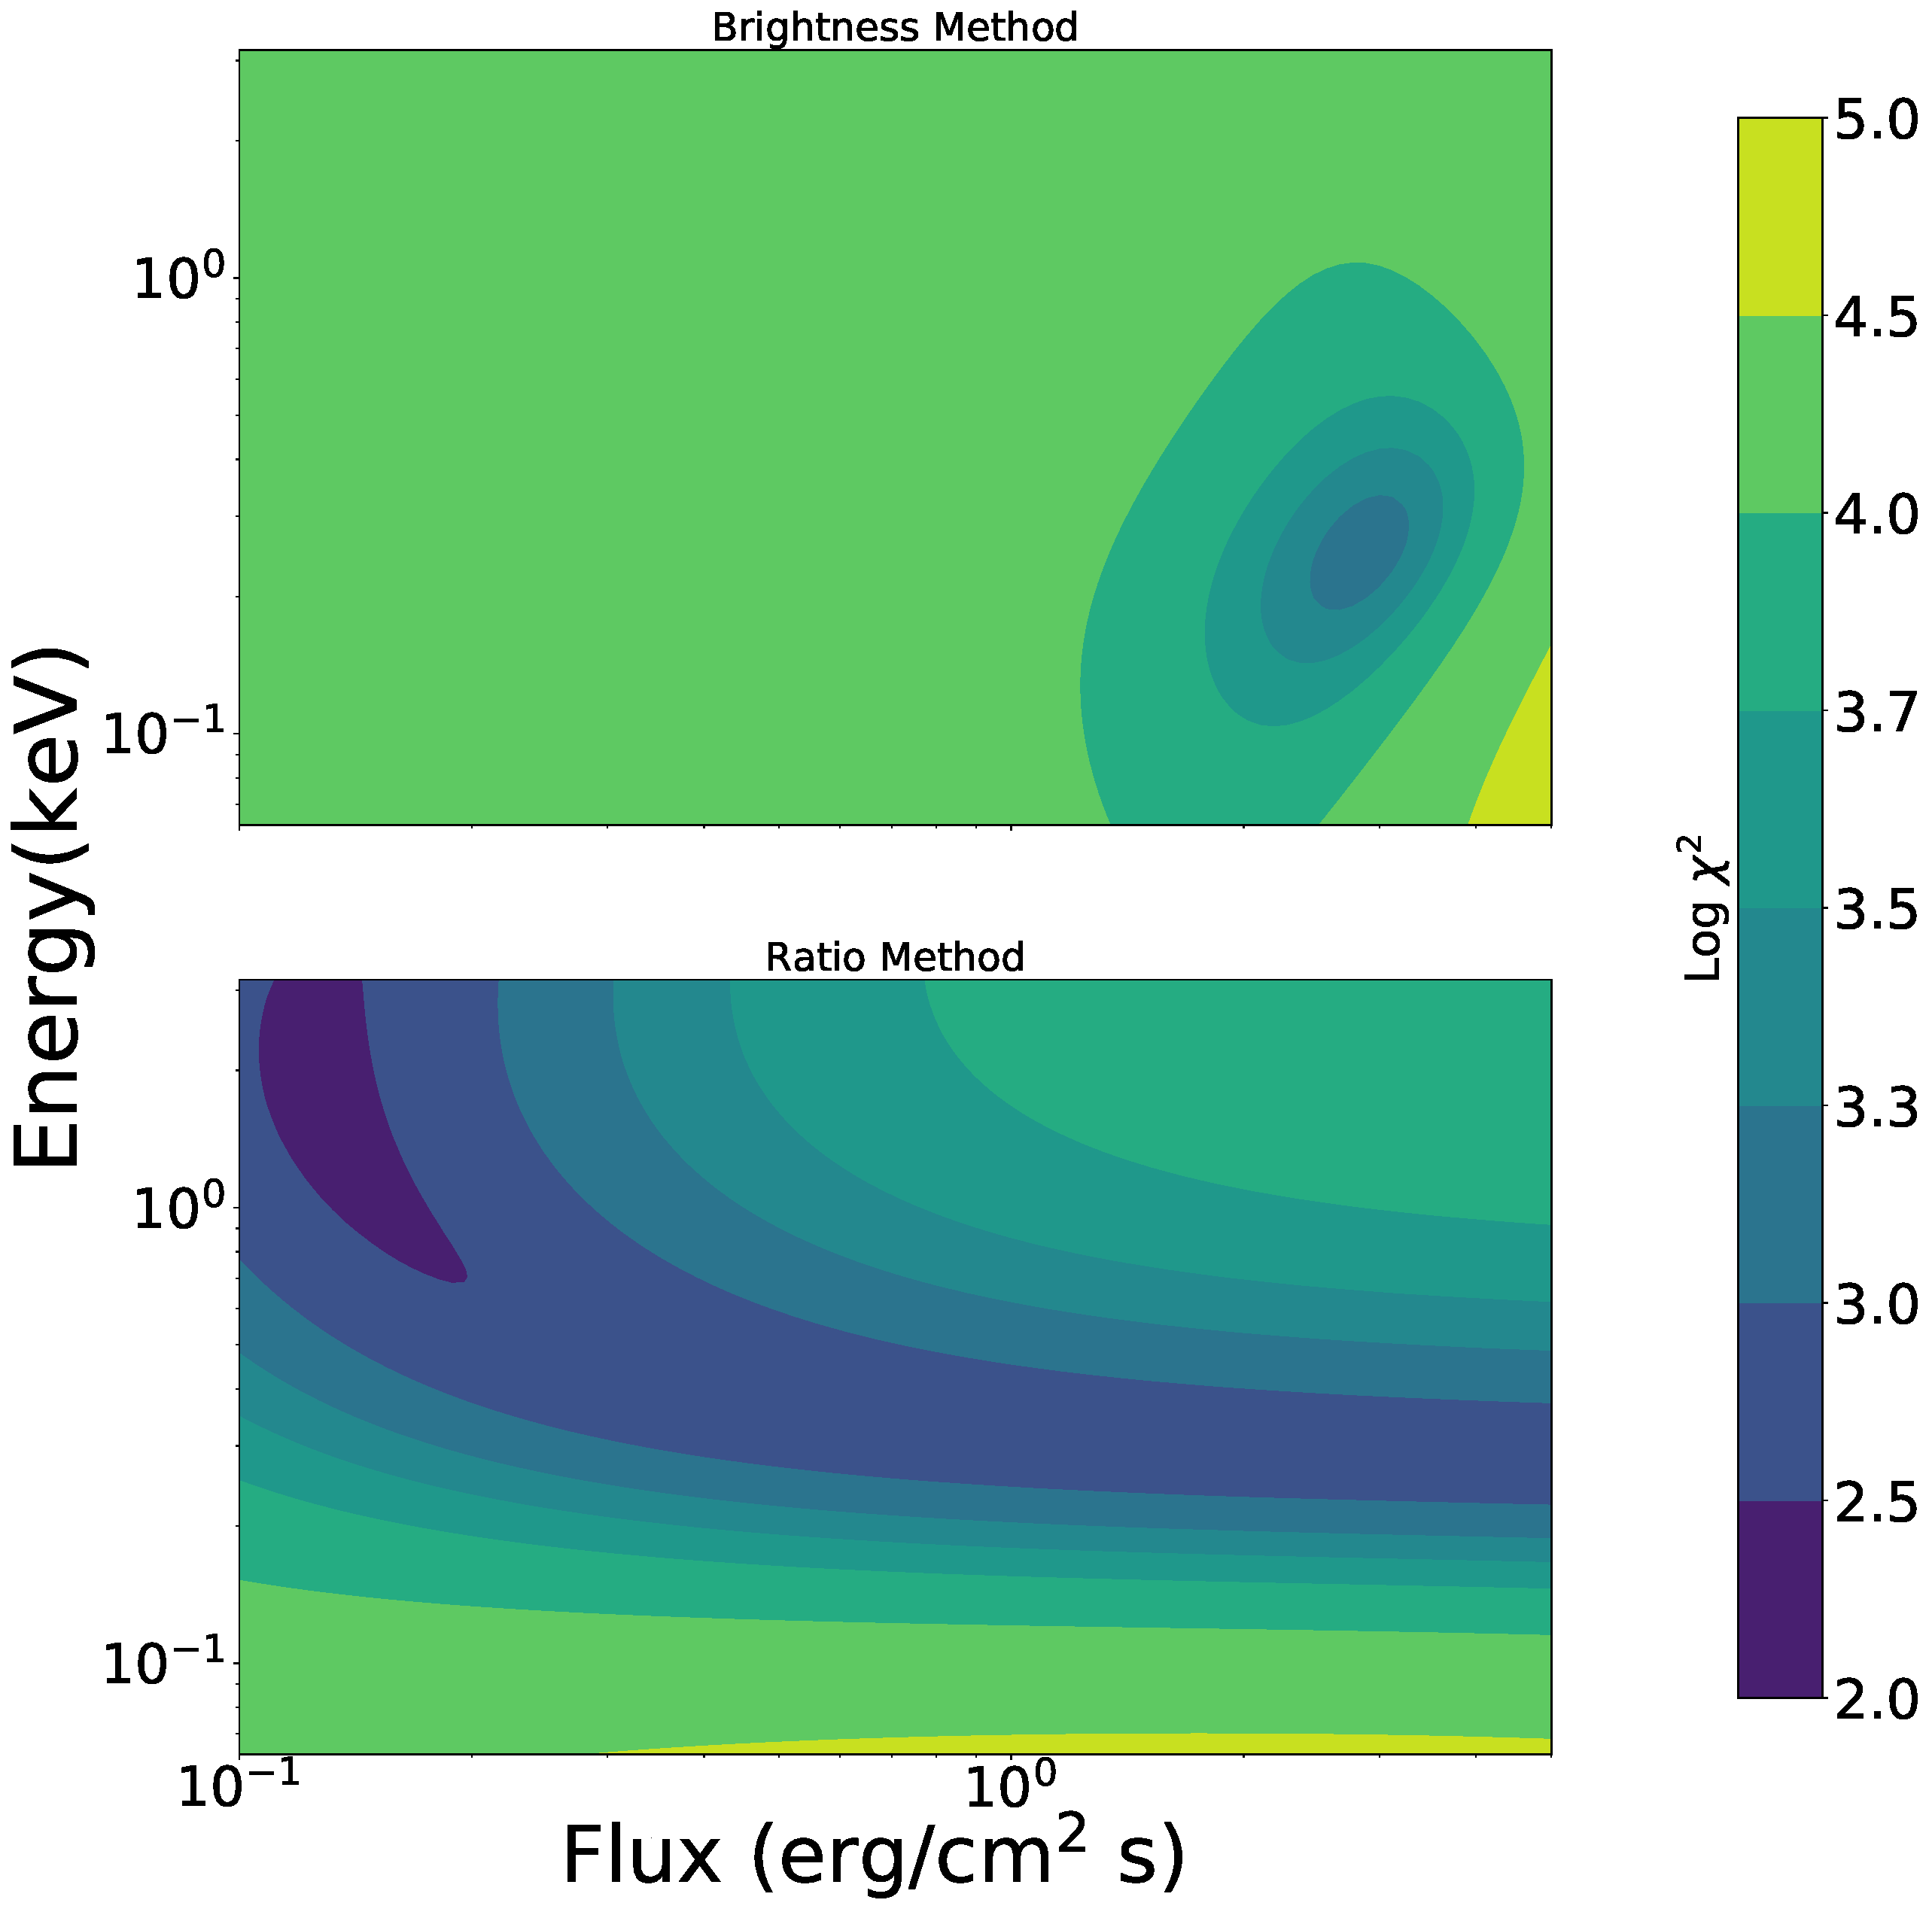
\includegraphics[width=32pc]{chi_b_vs_e_08.pdf}
	\caption{Log $\rm \chi^2$ as a function of characteristic energy and total energy flux at 00:08 LT, June 23,2015 using the brightness method (top) and the ratio method (bottom). Notice that for the brightness method, the minimum $\rm \chi^2$ is well-constrained for both energy and flux parameters.}
	\label{fig:chi_08}
\end{figure}
\begin{figure}
	\centering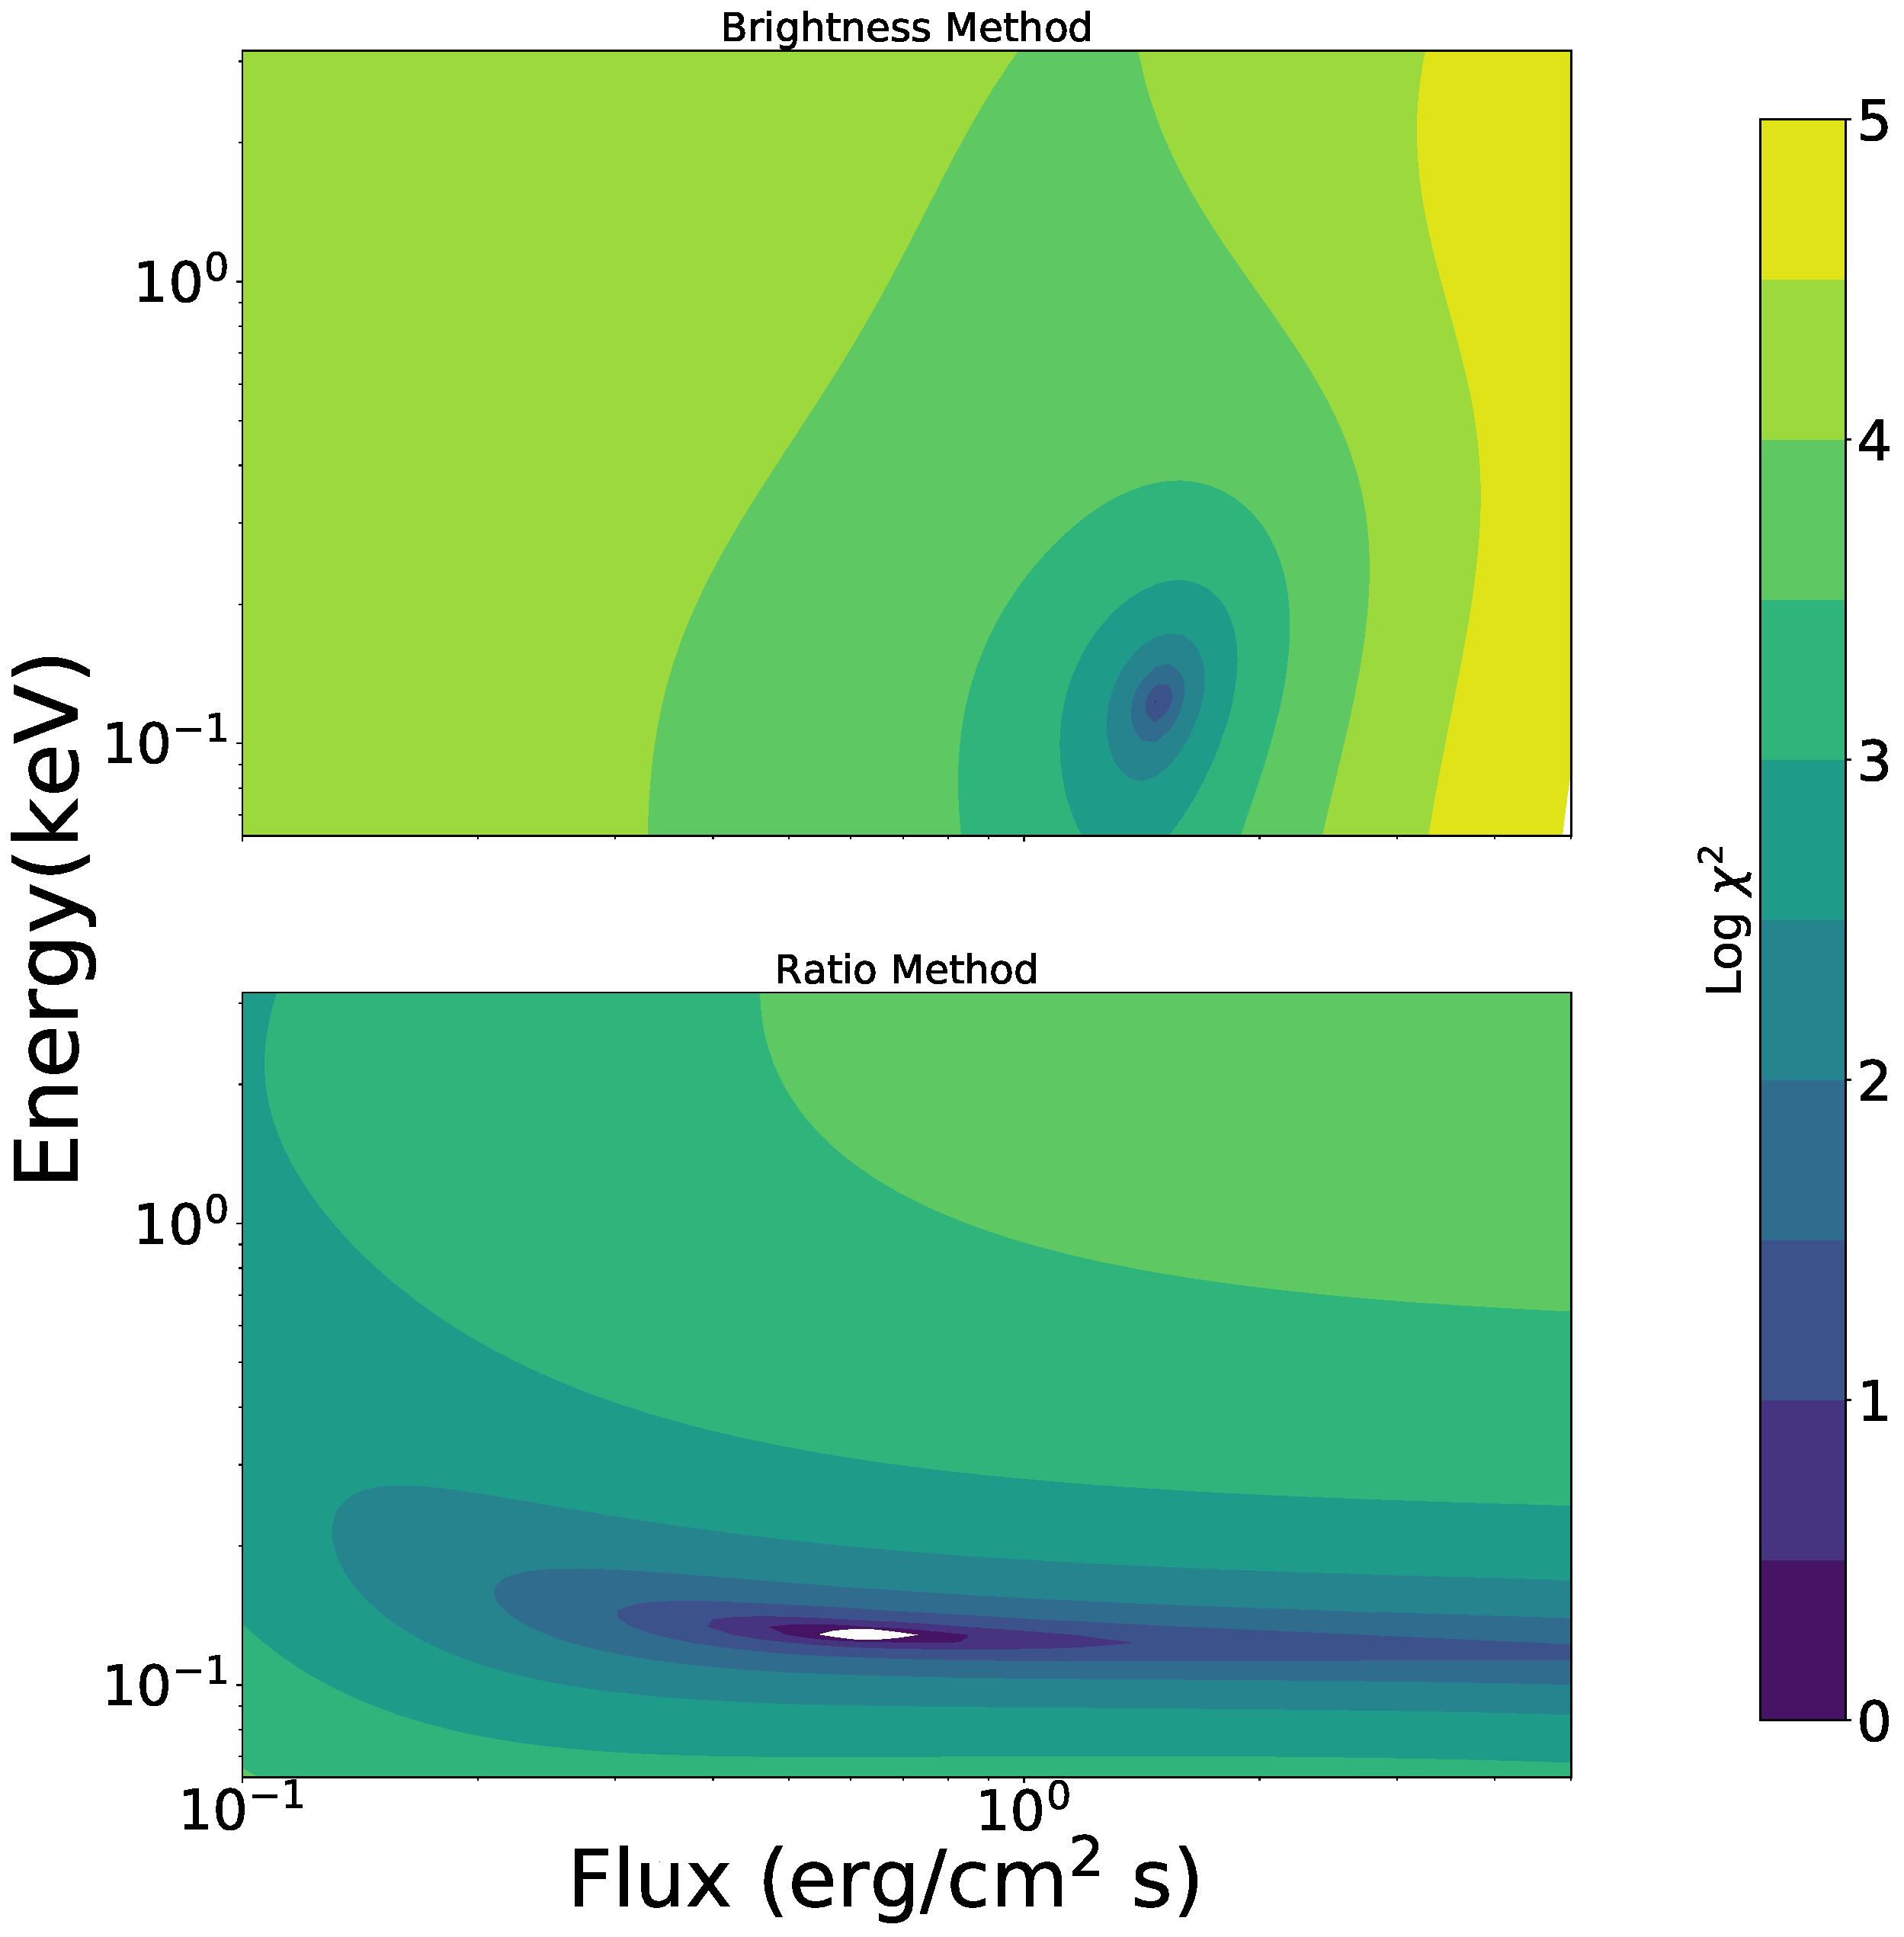
\includegraphics[width=32pc]{chi_b_vs_e_127.pdf}
	\caption{Log $\rm \chi^2$ as a function of characteristic energy and total energy flux at 01:27 LT, June 23,2015 using the brightness method (top) and the ratio method(bottom). Notice for the ratio method, the spread of $\rm \chi^2$ away from the minimum is much smaller than the brightness method.}
	\label{fig:chi_127}
\end{figure}
\begin{figure}
	\centering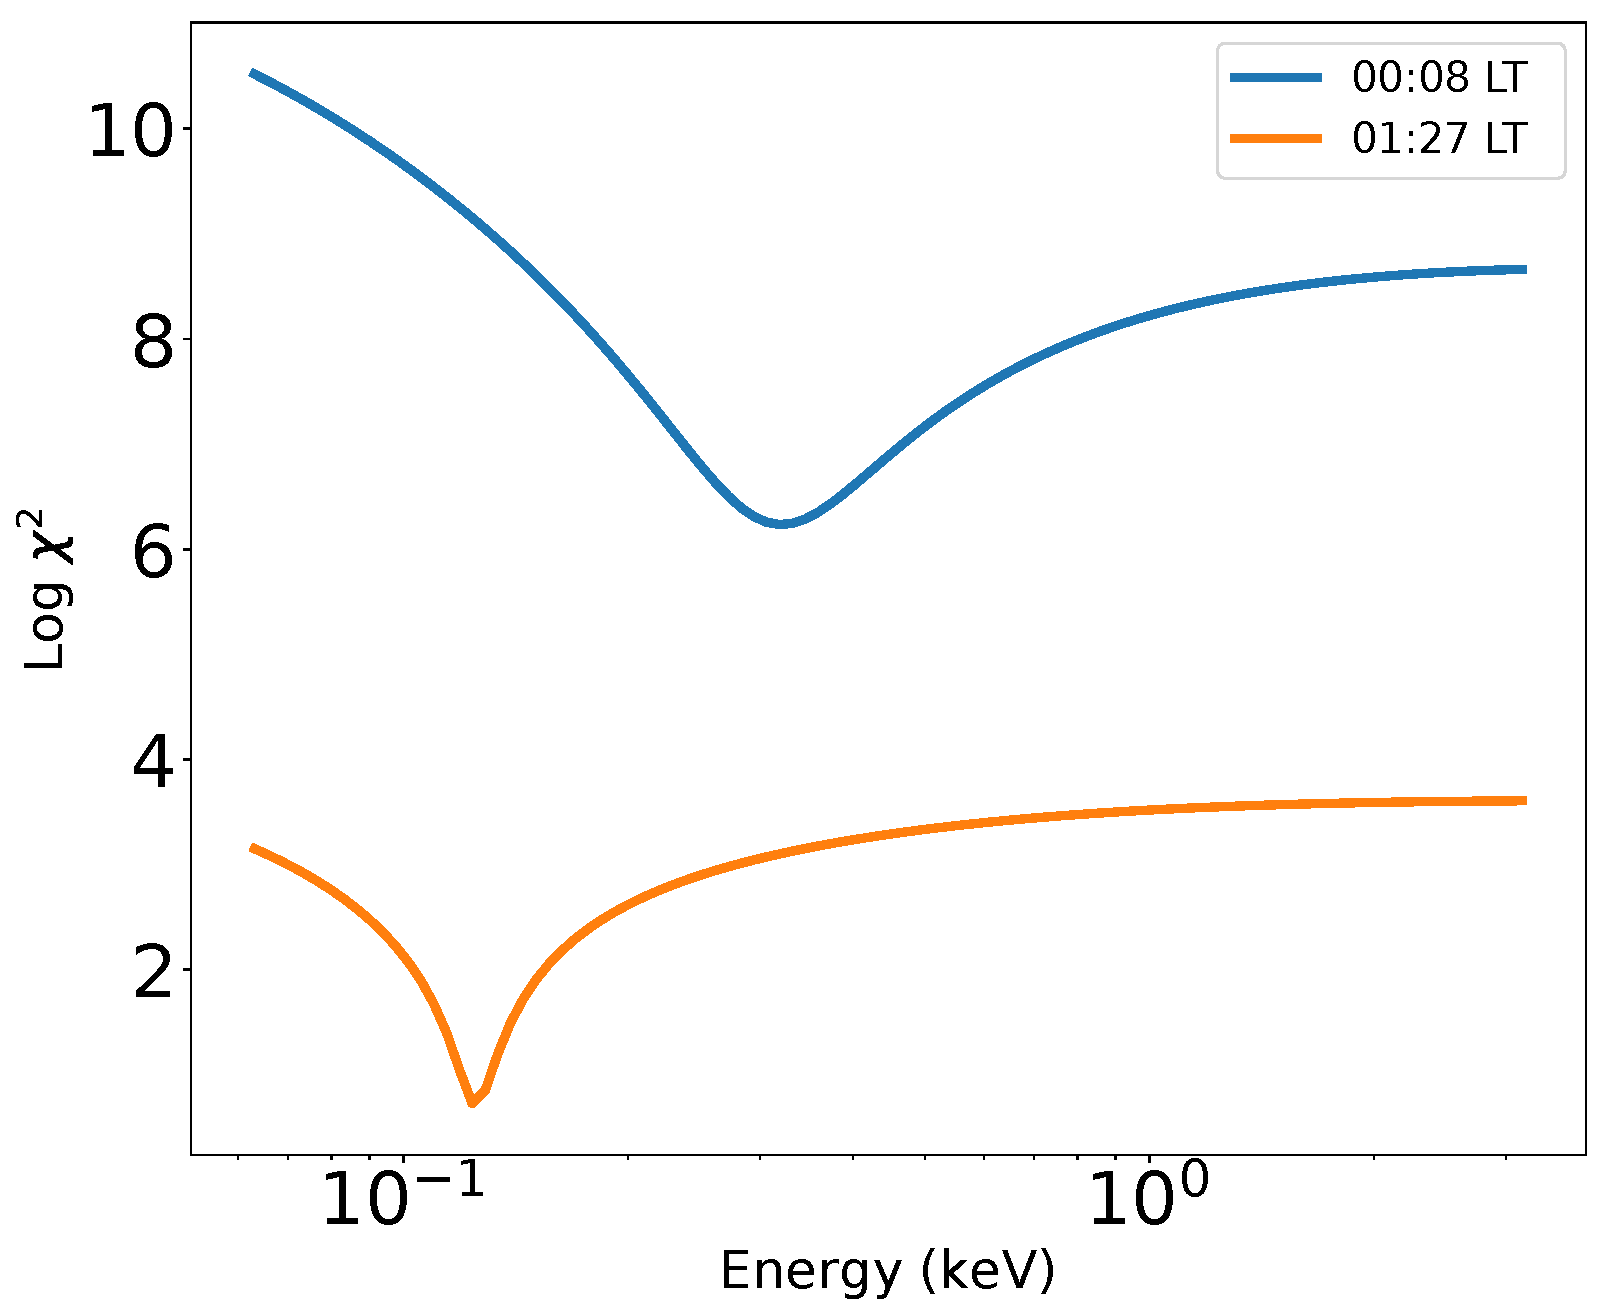
\includegraphics[width=32pc]{different_fl_evschi2.pdf}
	\caption{Log $\rm \chi^2$ as a function of characteristic energy at a constant flux of 1 erg $\rm cm^{-2} s^{-1}$ at 00:08 and 01:27 LT on June 23. The location of the minimum is used to estimate the energy in the first step of the hybrid method.}
	\label{fig:chi_hybrid}
\end{figure}
\begin{figure}
	\centering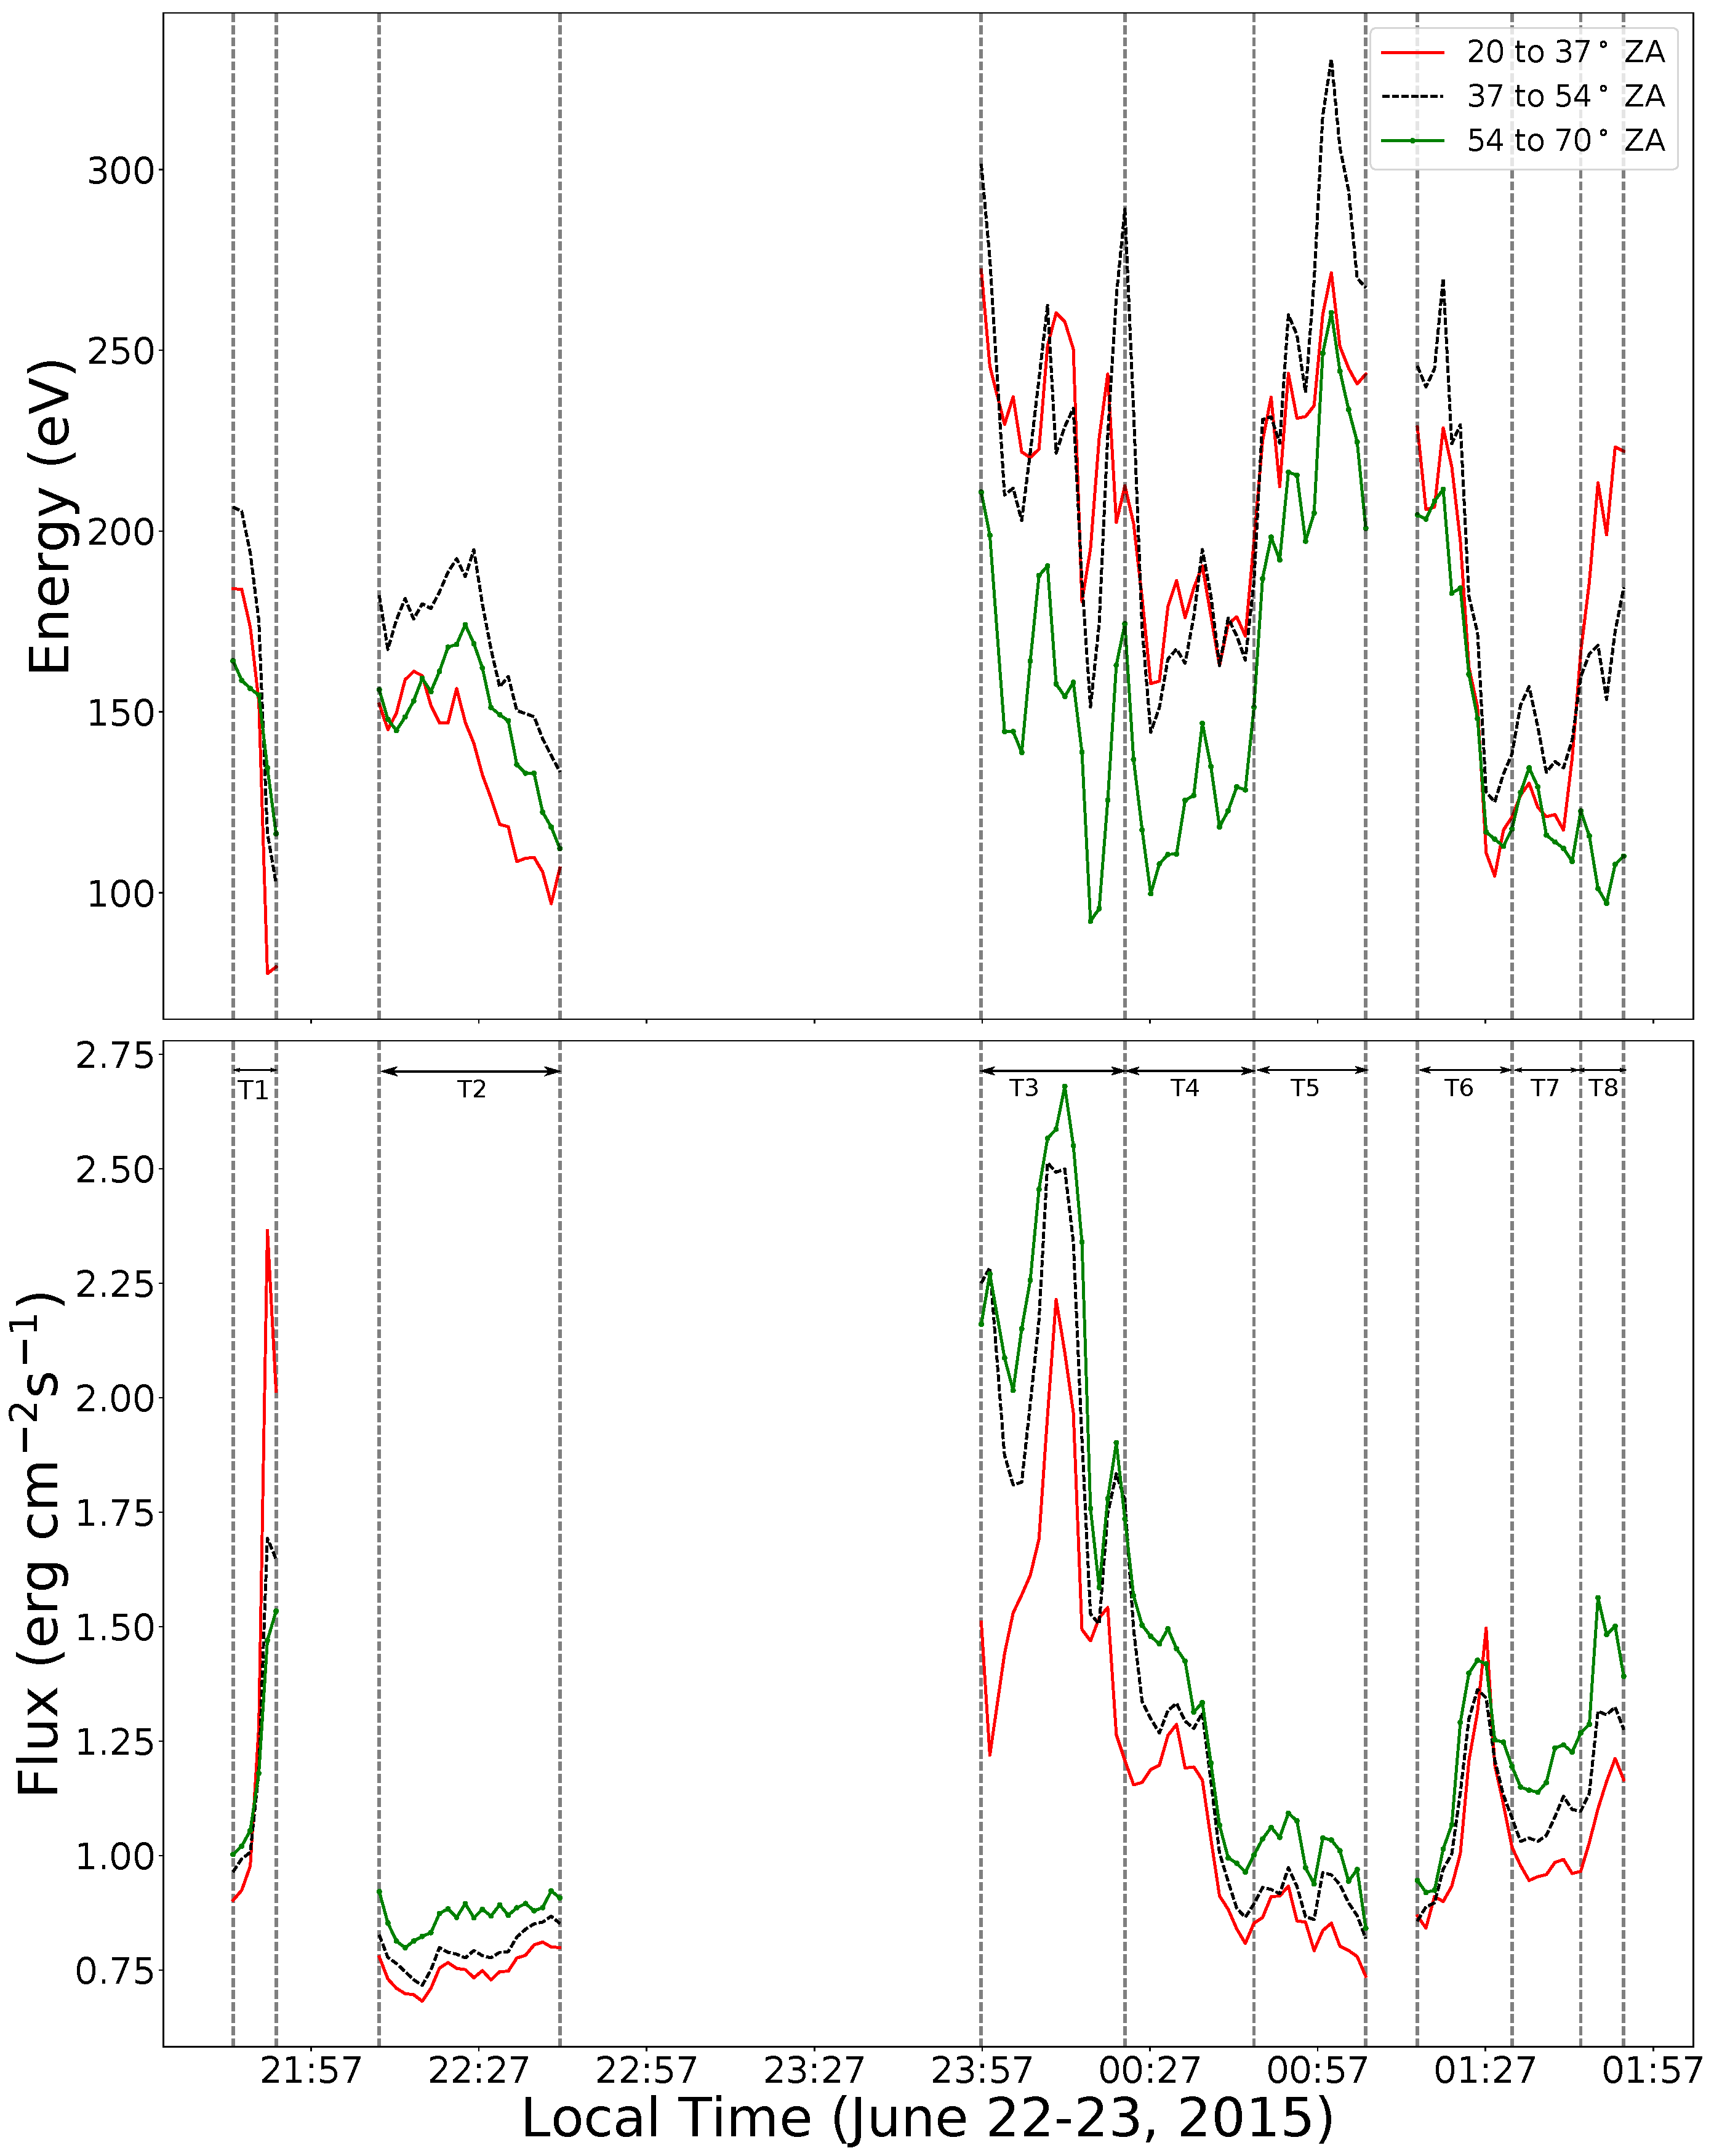
\includegraphics[width=30pc]{different_ld_m1_e_fl.pdf}
	\caption{Derived energies and energy fluxes using the brightness method at different look directions and times. Blank areas denote cloudy times based on the NeI 630.5 nm line shown in Figure \ref{feature:nbrg}. Notice the derived energies and flux show both temporal and zenith angle variations.}
	\label{fig:e_fl_la}
\end{figure}
\begin{figure}
	\centering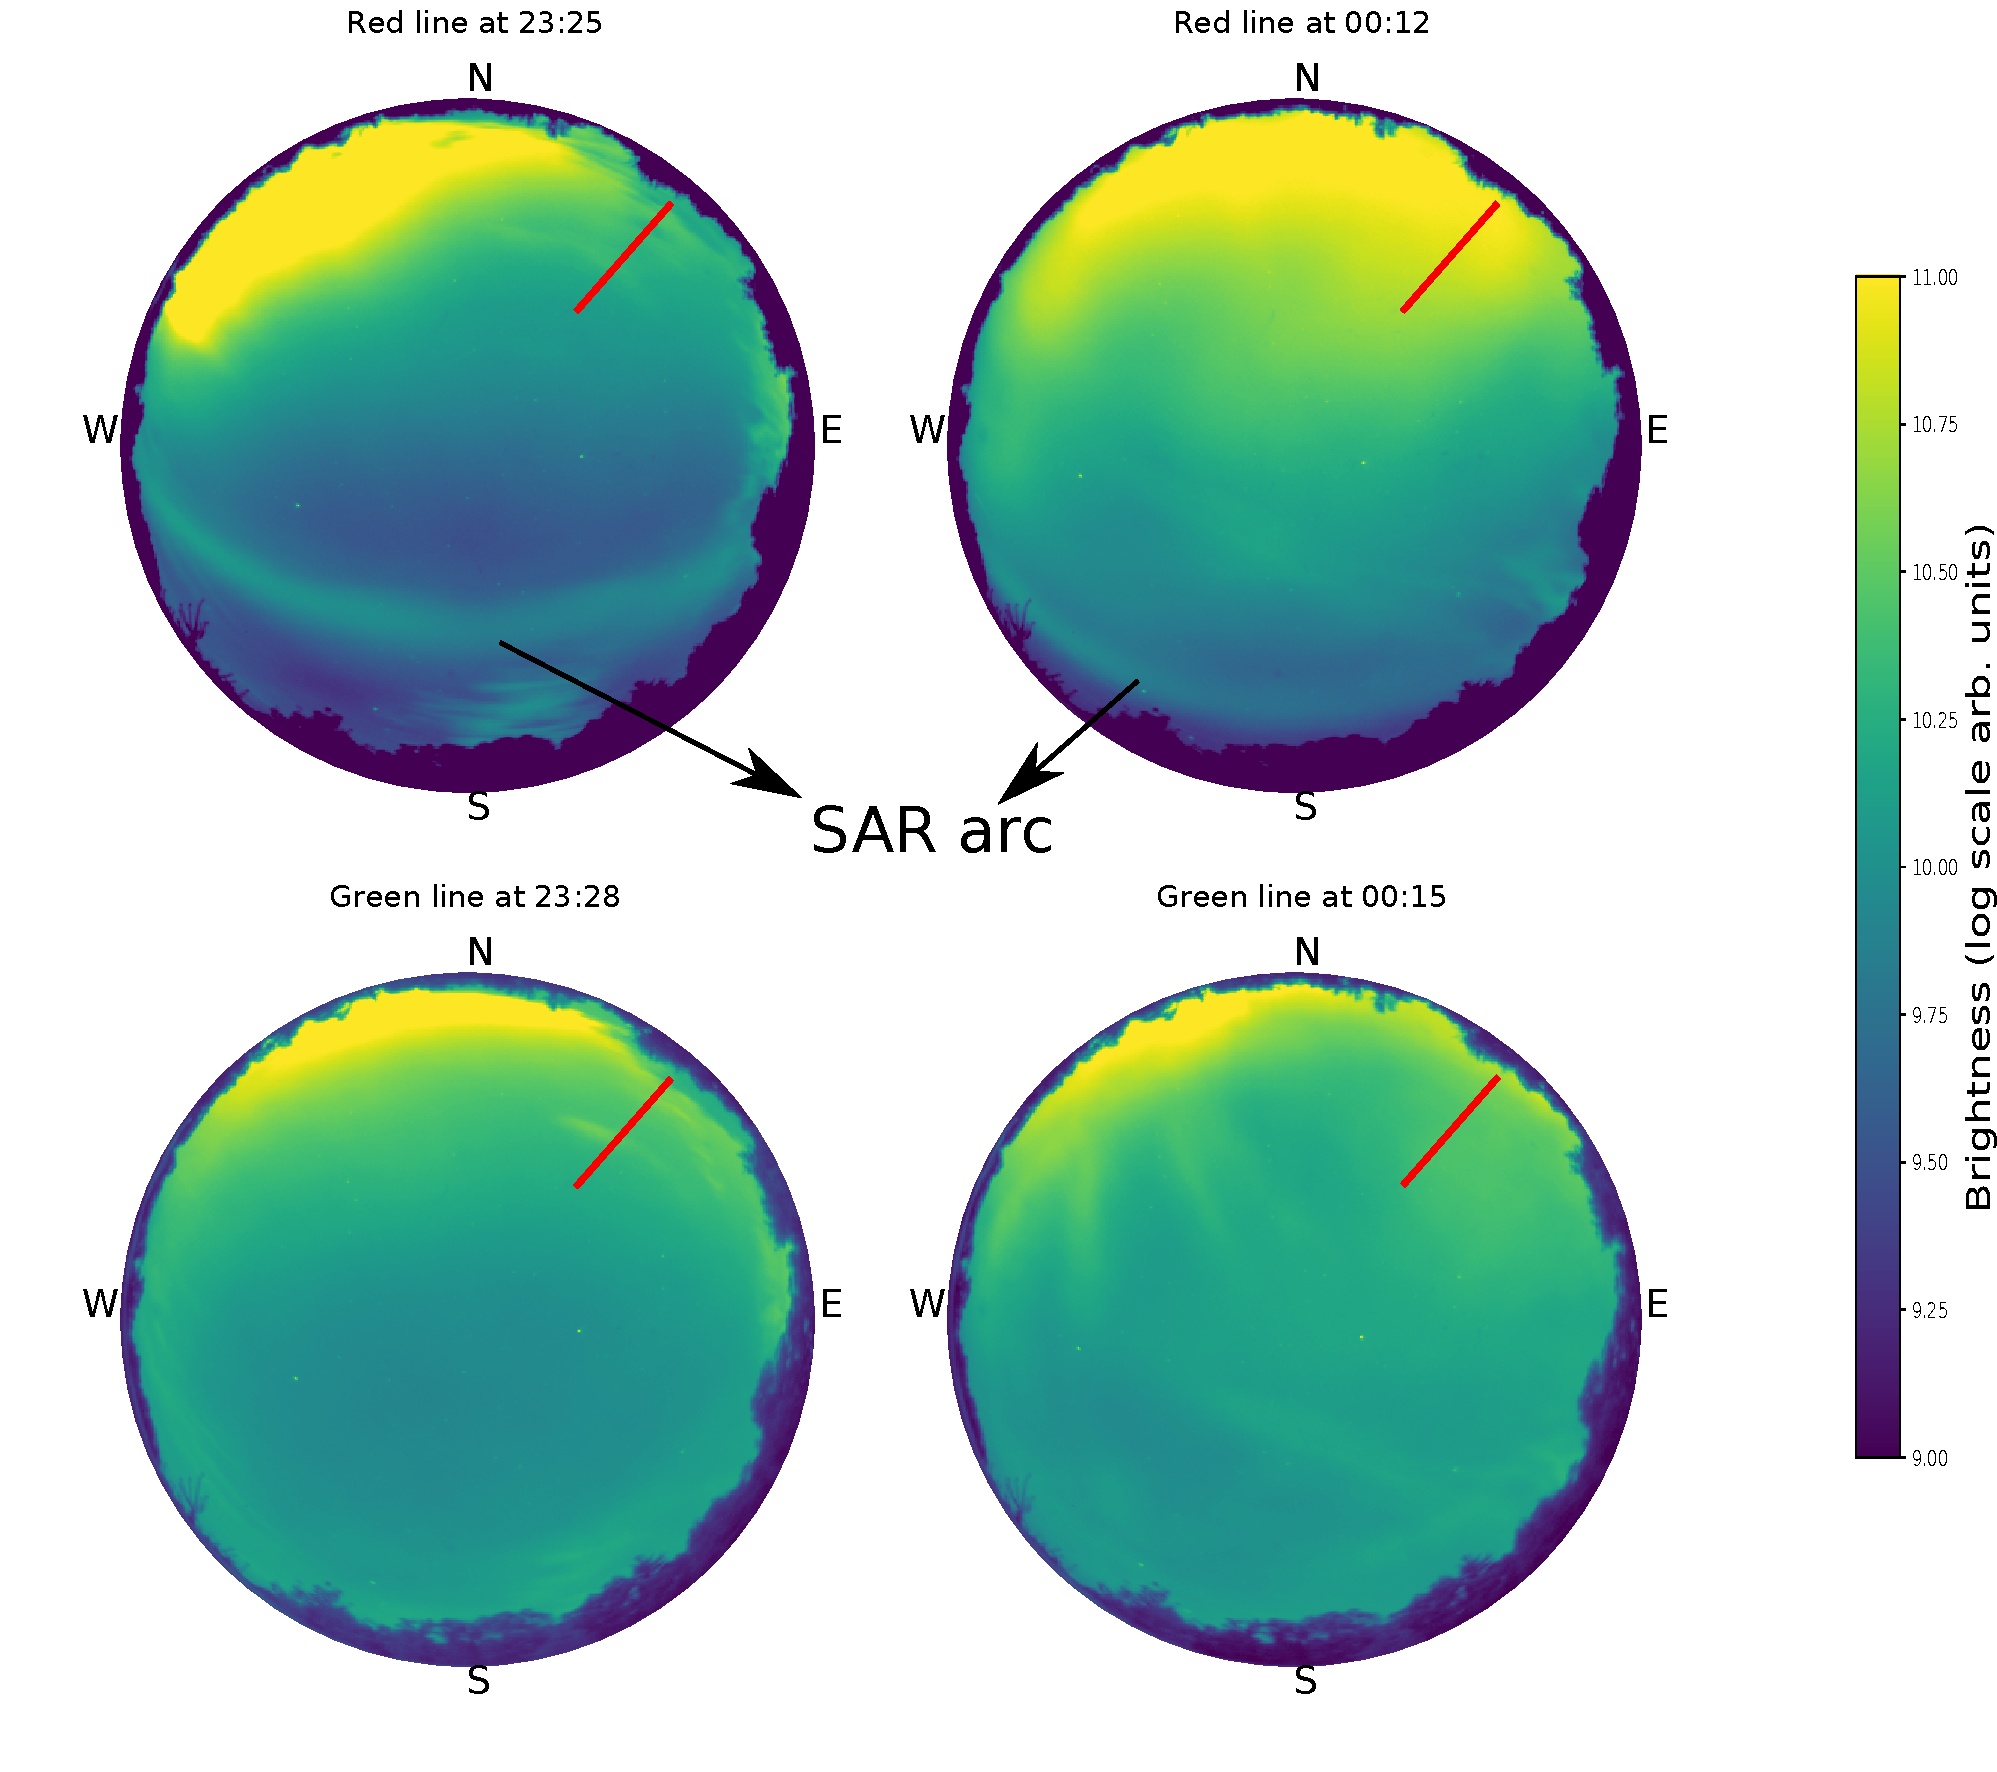
\includegraphics[width=35pc]{allsky.pdf}
	\caption{Boston University's all-sky images at Millstone Hill (approximately 10 miles southwest of Lowell, MA) in red and green lines for few selected times on June 22-23,2015. SAR arc was seen in the red line data towards the south (and moving southwards). HiT\&MIS's approximate FOV is shown with a black line on each image.}
	\label{fig:allsky}
\end{figure}



%The energy derived using the red to blue ratio and the $\chi^2$ minimization methods are comparable during most time period for measurements closest to the zenith. However, 


%\floatsetup[sidewaystable]{font=tiny}
%\begin{sidewaystable}
%\centering
%\caption{Energies derived at the times and look directions selected in Figure \ref{feature:nbrg} using three different minimization methods. For the derivation using the brightness and ratio methods, Equation \ref{eq:chi} was minimized by varying $E$ and $Q$ simultaneously to constrain model brightnesses or their ratios to measurements. For the simultaneous ratio method, Equation \ref{eq:chi} was minimized by varying $E$ to constrain the model brightness ratios to measurements. Then at the derived energy, the fluxes were derived by constraining the modeled red and green line brightness with measurements by varying $Q$ in Equation \ref{eq:chi}.}
%%\tablenotemark{a}}
%\centering
%\begin{tabular}{|l|l|l|l|l|l|l|l|l|l|l|}
%	\hline
%	\multicolumn{10}{|c|}{Energies ($eV$)}\\
%\hline
% Method&Brightness & Ratio & SR &    Brightness  & Ratio  &       SR  &Brightness  & Ratio  & SR \\
% \hline
% 
%Times&\multicolumn{3}{c|}{20$^\circ$-37$^\circ$ from zenith}& \multicolumn{3}{c|}{37$^\circ$-54$^\circ$ from zenith}& \multicolumn{3}{c|}{54$^\circ$-70$^\circ$ from zenith}\\
%\hline
%%T1   &    0.144$\pm$0.006 &    0.15$\pm$0.06 &     0.18$\pm$0.05 &    0.174$\pm$0.006 &      0.3$\pm$0.5 &     0.22$\pm$0.05 &  0.151$\pm$0.018 &    0.12$\pm$0.04 &     0.15$\pm$0.05 \\
%%T2   &  0.1257$\pm$0.0019 &    0.13$\pm$0.16 &   0.123$\pm$0.009 &  0.1652$\pm$0.0026 &    0.31$\pm$0.33 &   0.207$\pm$0.018 &  0.148$\pm$0.006 &    0.13$\pm$0.05 &   0.180$\pm$0.013 \\
%%T3   &  0.2449$\pm$0.0027 &  0.117$\pm$0.030 &     0.93$\pm$0.25 &  0.2293$\pm$0.0024 &  0.121$\pm$0.032 &     0.61$\pm$0.21 &  0.152$\pm$0.026 &  0.080$\pm$0.019 &   0.218$\pm$0.032 \\
%%T4   &  0.1917$\pm$0.0028 &  0.095$\pm$0.020 &     0.36$\pm$0.09 &  0.1899$\pm$0.0025 &  0.120$\pm$0.027 &     0.28$\pm$0.10 &  0.130$\pm$0.016 &  0.069$\pm$0.011 &   0.158$\pm$0.014 \\
%%T5   &    0.276$\pm$0.004 &    0.14$\pm$0.08 &     0.84$\pm$0.25 &  0.3075$\pm$0.0031 &    0.30$\pm$0.30 &     0.88$\pm$0.34 &  0.247$\pm$0.009 &    0.16$\pm$0.22 &     0.37$\pm$0.20 \\
%%T6   &  0.1833$\pm$0.0032 &    0.13$\pm$0.07 &     0.37$\pm$0.15 &    0.212$\pm$0.004 &    0.41$\pm$0.20 &     0.46$\pm$0.19 &  0.180$\pm$0.007 &    0.13$\pm$0.04 &     0.22$\pm$0.10 \\
%%T7   &  0.1251$\pm$0.0022 &    0.13$\pm$0.06 &   0.130$\pm$0.010 &  0.1457$\pm$0.0025 &    0.23$\pm$0.35 &   0.175$\pm$0.023 &  0.124$\pm$0.006 &  0.107$\pm$0.021 &   0.129$\pm$0.011 \\
%%T8   &    0.224$\pm$0.004 &    0.09$\pm$0.12 &     0.59$\pm$0.21 &    0.179$\pm$0.004 &    0.13$\pm$0.25 &     0.24$\pm$0.06 &    0.11$\pm$0.05 &    0.11$\pm$0.04 &   0.118$\pm$0.007 \\
%T1   &         147$\pm$35 &       132$\pm$15 &  620$\pm$110 &  170$\pm$40 &       159$\pm$14 &  710$\pm$70 &      151$\pm$34 &       144$\pm$24 &      600$\pm$400 \\
%T2   &         135$\pm$16 &    118$\pm$3 &      131$\pm$3 &         170$\pm$17 &    151$\pm$3 &         214$\pm$13 &      150$\pm$15 &        141$\pm$9 &      400$\pm$600 \\
%T3   &         230$\pm$31 &       204$\pm$27 &  700$\pm$1100 &         221$\pm$29 &       198$\pm$22 &      700$\pm$700 &      150$\pm$22 &       135$\pm$22 &      600$\pm$600 \\
%T4   &         179$\pm$24 &       164$\pm$23 &      600$\pm$900 &         181$\pm$24 &       165$\pm$20 &      600$\pm$500 &      126$\pm$18 &       123$\pm$20 &      600$\pm$400 \\
%T5   &         237$\pm$26 &       212$\pm$22 &  700$\pm$1500 &         262$\pm$29 &       233$\pm$20 &  700$\pm$1300 &      213$\pm$25 &       196$\pm$24 &  600$\pm$2600 \\
%T6   &         170$\pm$24 &       155$\pm$16 &      400$\pm$600 &         195$\pm$25 &       177$\pm$12 &  400$\pm$1300 &      164$\pm$22 &       154$\pm$19 &      500$\pm$900 \\
%T7   &         125$\pm$22 &        114$\pm$8 &          151$\pm$7 &         142$\pm$24 &        130$\pm$8 &         181$\pm$11 &      120$\pm$22 &       114$\pm$18 &  500$\pm$210 \\
%T8   &  200$\pm$40 &       183$\pm$26 &  700$\pm$1200 &         167$\pm$30 &       154$\pm$17 &  700$\pm$200 &      109$\pm$24 &       103$\pm$20 &         372$\pm$33 \\
%\hline
%\end{tabular}
%% \begin{tabular}{l c r}
%% \hline
%% %  Method  & Energy (keV) & Flux(erg/(cm$^2$ s)  \\
%% % \hline
%% % 630.0 nm/427.8 nm ratio  & 0.1$\pm$0.05 & 1.5$\pm$0.2   \\
%% %   630.0 nm/557.7 nm ratio  & 0.17$\pm$1.4 & 1.67$\pm$0.18   \\
%% %   $\chi^2$ &0.15$\pm$0.003 & 0.89$\pm$0.007\\
%% \end{tabular}
%\label{table:energy}
%\end{sidewaystable}
%\begin{sidewaystable}
%\centering
%\caption{Fluxes derived at the times and look directions selected in Figure \ref{feature:nbrg} using different methods. For the derivation using the brightness and ratio methods, Equation \ref{eq:chi} was minimized by varying $E$ and $Q$ simultaneously to constrain model brightnesses or their ratios to measurements. For the simultaneous ratio method, Equation \ref{eq:chi} was minimized by varying the energy ($E$) to constrain the model brightness ratios to measurements. Then at the derived energy, the fluxes were derived by constraining the modeled red and green line brightness with measurements by varying $Q$ in Equation \ref{eq:chi}.}
%	%\tablenotemark{a}}
%\centering
%\begin{tabular}{|l|l|l|l|l|l|l|l|l|l|}
%\hline
%\multicolumn{10}{|c|}{Fluxes ($erg$ $cm^{-2} s^{-1}$)}\\
%\hline
%Method $\rightarrow$ &Brightness & Ratio & SR &    Brightness  & Ratio  &       SR  &Brightness  & Ratio  & SR \\
%\hline
%
%Times&\multicolumn{3}{c|}{20$^\circ$-37$^\circ$ ZA}& \multicolumn{3}{c|}{37$^\circ$-54$^\circ$ ZA}& \multicolumn{3}{c|}{54$^\circ$-70$^\circ$ ZA}\\
%\hline
%%T1   &  1.593$\pm$0.034 &    1.77$\pm$0.25 &     1.85$\pm$0.22 &  1.386$\pm$0.013 &      2.4$\pm$1.5 &     1.61$\pm$0.19 &    1.33$\pm$0.26 &    1.24$\pm$0.04 &     1.39$\pm$0.06 \\
%%T2   &  0.814$\pm$0.006 &    0.91$\pm$0.33 &   0.827$\pm$0.027 &  0.870$\pm$0.007 &      1.2$\pm$0.6 &     1.02$\pm$0.04 &  0.945$\pm$0.033 &    0.92$\pm$0.05 &   0.951$\pm$0.015 \\
%%T3   &  1.909$\pm$0.009 &    1.29$\pm$0.16 &       3.6$\pm$0.4 &  2.314$\pm$0.013 &    1.71$\pm$0.21 &       3.6$\pm$0.4 &    2.47$\pm$0.17 &  2.000$\pm$0.019 &     2.58$\pm$0.04 \\
%%T4   &  1.235$\pm$0.010 &    0.90$\pm$0.08 &     1.88$\pm$0.30 &  1.378$\pm$0.009 &    1.13$\pm$0.13 &     1.94$\pm$0.21 &    1.46$\pm$0.07 &  1.210$\pm$0.011 &   1.490$\pm$0.027 \\
%%T5   &  0.956$\pm$0.008 &    0.65$\pm$0.24 &       2.6$\pm$0.6 &  1.042$\pm$0.009 &      1.0$\pm$0.7 &       2.9$\pm$0.7 &    1.15$\pm$0.06 &    0.90$\pm$0.22 &   1.170$\pm$0.021 \\
%%T6   &  1.198$\pm$0.011 &      1.1$\pm$0.4 &       2.0$\pm$0.6 &  1.241$\pm$0.013 &      2.3$\pm$0.7 &       2.3$\pm$0.5 &    1.31$\pm$0.05 &    1.18$\pm$0.04 &   1.342$\pm$0.029 \\
%%T7   &  1.041$\pm$0.010 &    1.08$\pm$0.29 &     1.09$\pm$0.04 &  1.150$\pm$0.013 &      1.7$\pm$0.7 &     1.32$\pm$0.10 &    1.29$\pm$0.09 &  1.251$\pm$0.021 &   1.334$\pm$0.029 \\
%%T8   &  1.252$\pm$0.017 &      0.8$\pm$0.6 &       2.7$\pm$0.7 &  1.372$\pm$0.013 &      1.2$\pm$0.7 &     1.75$\pm$0.20 &    1.57$\pm$0.13 &    1.60$\pm$0.04 &   1.600$\pm$0.033 \\
%T1   &   1.39$\pm$0.19 &    1.581$\pm$0.01 &    0.26$\pm$0.09 &   1.22$\pm$0.12 &    1.30$\pm$0.01 &    0.32$\pm$0.23 &   1.18$\pm$0.12 &    1.30$\pm$0.01 &    0.11$\pm$0.02 \\
%T2   &   0.75$\pm$0.04 &  0.82$\pm$0.01 &    0.81$\pm$0.19 &   0.79$\pm$0.04 &  0.89$\pm$0.001 &      2.3$\pm$0.4 &   0.87$\pm$0.04 &  0.94$\pm$0.01 &    0.12$\pm$0.02 \\
%T3   &   1.64$\pm$0.11 &      1.85$\pm$0.04 &    0.06$\pm$0.04 &   2.02$\pm$0.12 &    2.27$\pm$0.028 &  0.064$\pm$0.025 &   2.20$\pm$0.14 &      2.50$\pm$0.04 &    0.035$\pm$0.012 \\
%T4   &   1.10$\pm$0.07 &    1.24$\pm$0.014 &  0.041$\pm$0.019 &   1.24$\pm$0.07 &    1.38$\pm$0.016 &  0.045$\pm$0.015 &   1.33$\pm$0.08 &    1.45$\pm$0.008 &    0.026$\pm$0.005 \\
%T5   &   0.85$\pm$0.05 &    0.91$\pm$0.015 &    0.07$\pm$0.07 &   0.92$\pm$0.05 &    0.98$\pm$0.015 &    0.08$\pm$0.10 &   1.02$\pm$0.06 &    1.09$\pm$0.017 &      0.06$\pm$0.11 \\
%T6   &   1.09$\pm$0.07 &    1.19$\pm$0.009 &  0.08$\pm$0.022 &   1.12$\pm$0.07 &    1.20$\pm$0.008 &      1.1$\pm$2.7 &   1.20$\pm$0.07 &    1.29$\pm$0.010 &    0.05$\pm$0.026 \\
%T7   &   0.97$\pm$0.07 &  1.06$\pm$0.0013 &  0.12$\pm$0.024 &   1.07$\pm$0.07 &  1.20$\pm$0.0017 &  0.11$\pm$0.018 &   1.19$\pm$0.09 &  1.30$\pm$0.03 &  0.03$\pm$0.0023 \\
%T8   &   1.11$\pm$0.09 &    1.20$\pm$0.021 &    0.05$\pm$0.04 &   1.24$\pm$0.10 &    1.40$\pm$0.008 &  0.045$\pm$0.006 &   1.42$\pm$0.12 &  1.57$\pm$0.02 &  0.03$\pm$0.002 \\
%\hline
%\end{tabular}
%\label{table:flux}
%\end{sidewaystable}
% \begin{figure}
%  \centering\includegraphics[width=20pc]{e_der.pdf}
%  \caption{Energy derived by comparing observed brightness ratios to the modeled brightnesses ratios. The different measured brightness ratios are shown on top and color on the energy derivation plots (bottom) indicates which brightness ratio (on top) was used for derivation, and
%  the color shades indicates the $\pm$ 1$\sigma$ uncertainty.}
%  \label{fig:ej22}
%  \end{figure}
%  %%%%%%%%%%%%%%%%%%%%%%%%%%%%%%
%  \begin{figure}
%  \centering\includegraphics[width=20pc]{fl_der.pdf}
%  \caption{Top: The 427.8 nm brightness, which is proportional to the precipitating flux [cite]. Bottom: Fluxes derived by comparing the observed brightness to the modeled brightnesses at a fixed energy value derived in Figure \ref{fig:ej22} (bottom) for that particular time. The color shade indicates the
%  $\pm$ 1$\sigma$ uncertainty.}
%  \label{fig:flj22}
%  \end{figure}
%  %%%%%%%%%%%%%%%%%%%%%%%%%5
%   \begin{figure}
%  \centering\includegraphics[width=20pc]{fl_e.pdf}
%  \caption{Flux and energy derived by using the $\chi^2$ constraining (see equation \ref{eq:chi}) of the observed brightness to the modeled brightnesses. Since it was partly cloudy during our observation time, a time period
%  where all the emission features increased in brightness simultaneously (Auroral time 1 in the figure) and was cloudless is shown. (Need to show more times like this? May be need to show 630.5 ``cloud tracer`` line too?)}
%  \label{fig:fle}
%  \end{figure}
\begin{sidewaystable}
	\caption{Average (temporal) energies and fluxes derived at the time periods (T1 to T8) and look directions selected in Figure \ref{feature:nbrg} using the brightness method. In this method, $\chi^2$ in Equation \ref{eq:chi} was minimized by constraining the energy ($E$) and the flux ($Q$) parameters simultaneously by comparing model brightness to measurements.}
	\begin{tabular}{|l|l|l|l|l|l|l|}
		\hline
		Times& \multicolumn{3}{c|}{Energy (eV)} & \multicolumn{3}{c|}{Flux (erg $\rm cm^{-2} s^{-1}$)}\\ 
		\hline
		ZA $\rightarrow$& 20$^\circ$-37$^\circ$                  & 37$^\circ$-54$^\circ$                  &54$^\circ$-70$^\circ$                &20$^\circ$-37$^\circ$               &37$^\circ$-54$^\circ$                &54$^\circ$-70$^\circ$               \\	 \hline 
		
		
		T1   &         147$\pm$35 &         170$\pm$40 &      151$\pm$34 &   1.39$\pm$0.19 &   1.22$\pm$0.12 &   1.18$\pm$0.12 \\
		T2   &         135$\pm$16 &         170$\pm$17 &      150$\pm$15 &   0.75$\pm$0.04 &   0.79$\pm$0.04 &   0.87$\pm$0.04 \\
		T3   &         230$\pm$31 &         221$\pm$29 &      150$\pm$22 &   1.64$\pm$0.11 &   2.02$\pm$0.12 &   2.20$\pm$0.14 \\
		T4   &         179$\pm$24 &         181$\pm$24 &      126$\pm$18 &   1.10$\pm$0.07 &   1.24$\pm$0.07 &   1.33$\pm$0.08 \\
		T5   &         237$\pm$26 &         262$\pm$29 &      213$\pm$25 &   0.85$\pm$0.05 &   0.92$\pm$0.05 &   1.02$\pm$0.06 \\
		T6   &         170$\pm$24 &         195$\pm$25 &      164$\pm$22 &   1.09$\pm$0.07 &   1.12$\pm$0.07 &   1.20$\pm$0.07 \\
		T7   &         125$\pm$22 &         142$\pm$24 &      120$\pm$22 &   0.97$\pm$0.07 &   1.07$\pm$0.07 &   1.19$\pm$0.09 \\
		T8   &         200$\pm$40 &         167$\pm$30 &      109$\pm$24 &   1.11$\pm$0.09 &   1.24$\pm$0.10 &   1.42$\pm$0.12 \\
		\hline
	\end{tabular}
	\label{table:efl_look}		
\end{sidewaystable}

%------------------------------------------------



%Aliquam interdum pellentesque scelerisque. Sed tincidunt suscipit purus,compared to climatological HmF2 id aliquet nulla vehicula quis. Duis sed nisl lorem. Vivamus erat ante, dignissim et aliquam vel, adipiscing vitae magna. Cras id dapibus metus. Cum sociis natoque penatibus et magnis dis parturient montes, nascetur ridiculus mus. Proin ut lectus ut nisi congue ullamcorper. Ut ac turpis ligula. Sed faucibus bibendum nunc eget gravida.

%------------------------------------------------

\section{Discussion}
The Millstone Hill ISR radar was not observing and no ISR generated plasma profiles were available for our observation period. Thus, we used a digisonde \citep{giro} measurements at Westford, MA during our observation period (solid black line in Figure \ref{fig:digi}) for comparison. The F2 peak height obtaned from the digisonde measurements shows a rising hmF2 compared to the same period one day earlier (geomagnetically quiet time, Figure \ref{fig:digi}). This rise in hmF2 can also be caused by changes in either electric field strengths, winds or temperature. However, there is complete loss of radio signal in the digisonde data for most of our auroral observation period (from $\approx$ 22 LT June 22 to 02 LT June 23 in Figure \ref{fig:digi}). This can be attributed to the absorption of radio waves by excess E-region ionization caused by electron precipitation \citep{pallamraju_2011}. We therefore assumed the changes in brightnesses were due to auroral electrons. Additionally, since the low energy electrons are stopped at higher altitudes \citep{rees_1963} the observed rise in
hmF2 compared to the quiet day (Figure \ref{fig:digi}) is consistent with our results indicating that the energies of precipitating electrons were soft ($<$ 600 eV).

%The measurements  suffers from the fact that 
Since the emission features we observed peak at different altitudes, the measurements trace a wider range of magnetic and geographic latitudes with increasing zenith angles for emissions at higher altitudes (Figure \ref{fig:elayer}). The results for higher zenith angles, therefore, might be less accurate compared to the results at lower zenith angles. Similarly, our observations were also not aligned along the magnetic zenith. So this could limit the accuracy of the results derived for off-magnetic zenith measurements \citep{grubbs_multi_spec}. In addition, IRI90-generated plasma (election and ion) density and plasma temperature profiles could be inaccurate during storm-time \citep{iri_storm}. Similarly, MSIS00 neutral densities during geomagnetic storms can be up to 40\% inaccurate \citep{fang_variations_2012}. This adds uncertainty to the brightness estimates using the GLOW model. In the present study, the uncertainties in the model were not quantified and the uncertainties in energy and energy flux estimates were purely statistical arising from the minimization of $\chi^2$ in Equation \ref{eq:chi}. Hence, the actual uncertainties in the derived energies and fluxes could be much higher than reported in this paper.    


%   \begin{figure}
%  \centering\includegraphics[width=20pc]{rees_r_data.pdf}
%  \caption{OI 630 nm to $N_{2}^+$ 427.8 nm brightness ratio as a function of $N_{2}^+$ 427.8 nm brightness from GLOW model (solid lines) and data (red points) during Auroral period 1 on
%  Figure \ref{fig:fle} for various energies. This plot is similar to the ratio and brightness plots shown in \citet{rees_1974}, but with measurement data added to the plot.}
%  \label{fig:rees_r_d}
%  \end{figure}
%%%%% The GAMBIT plot

\begin{figure}
	\centering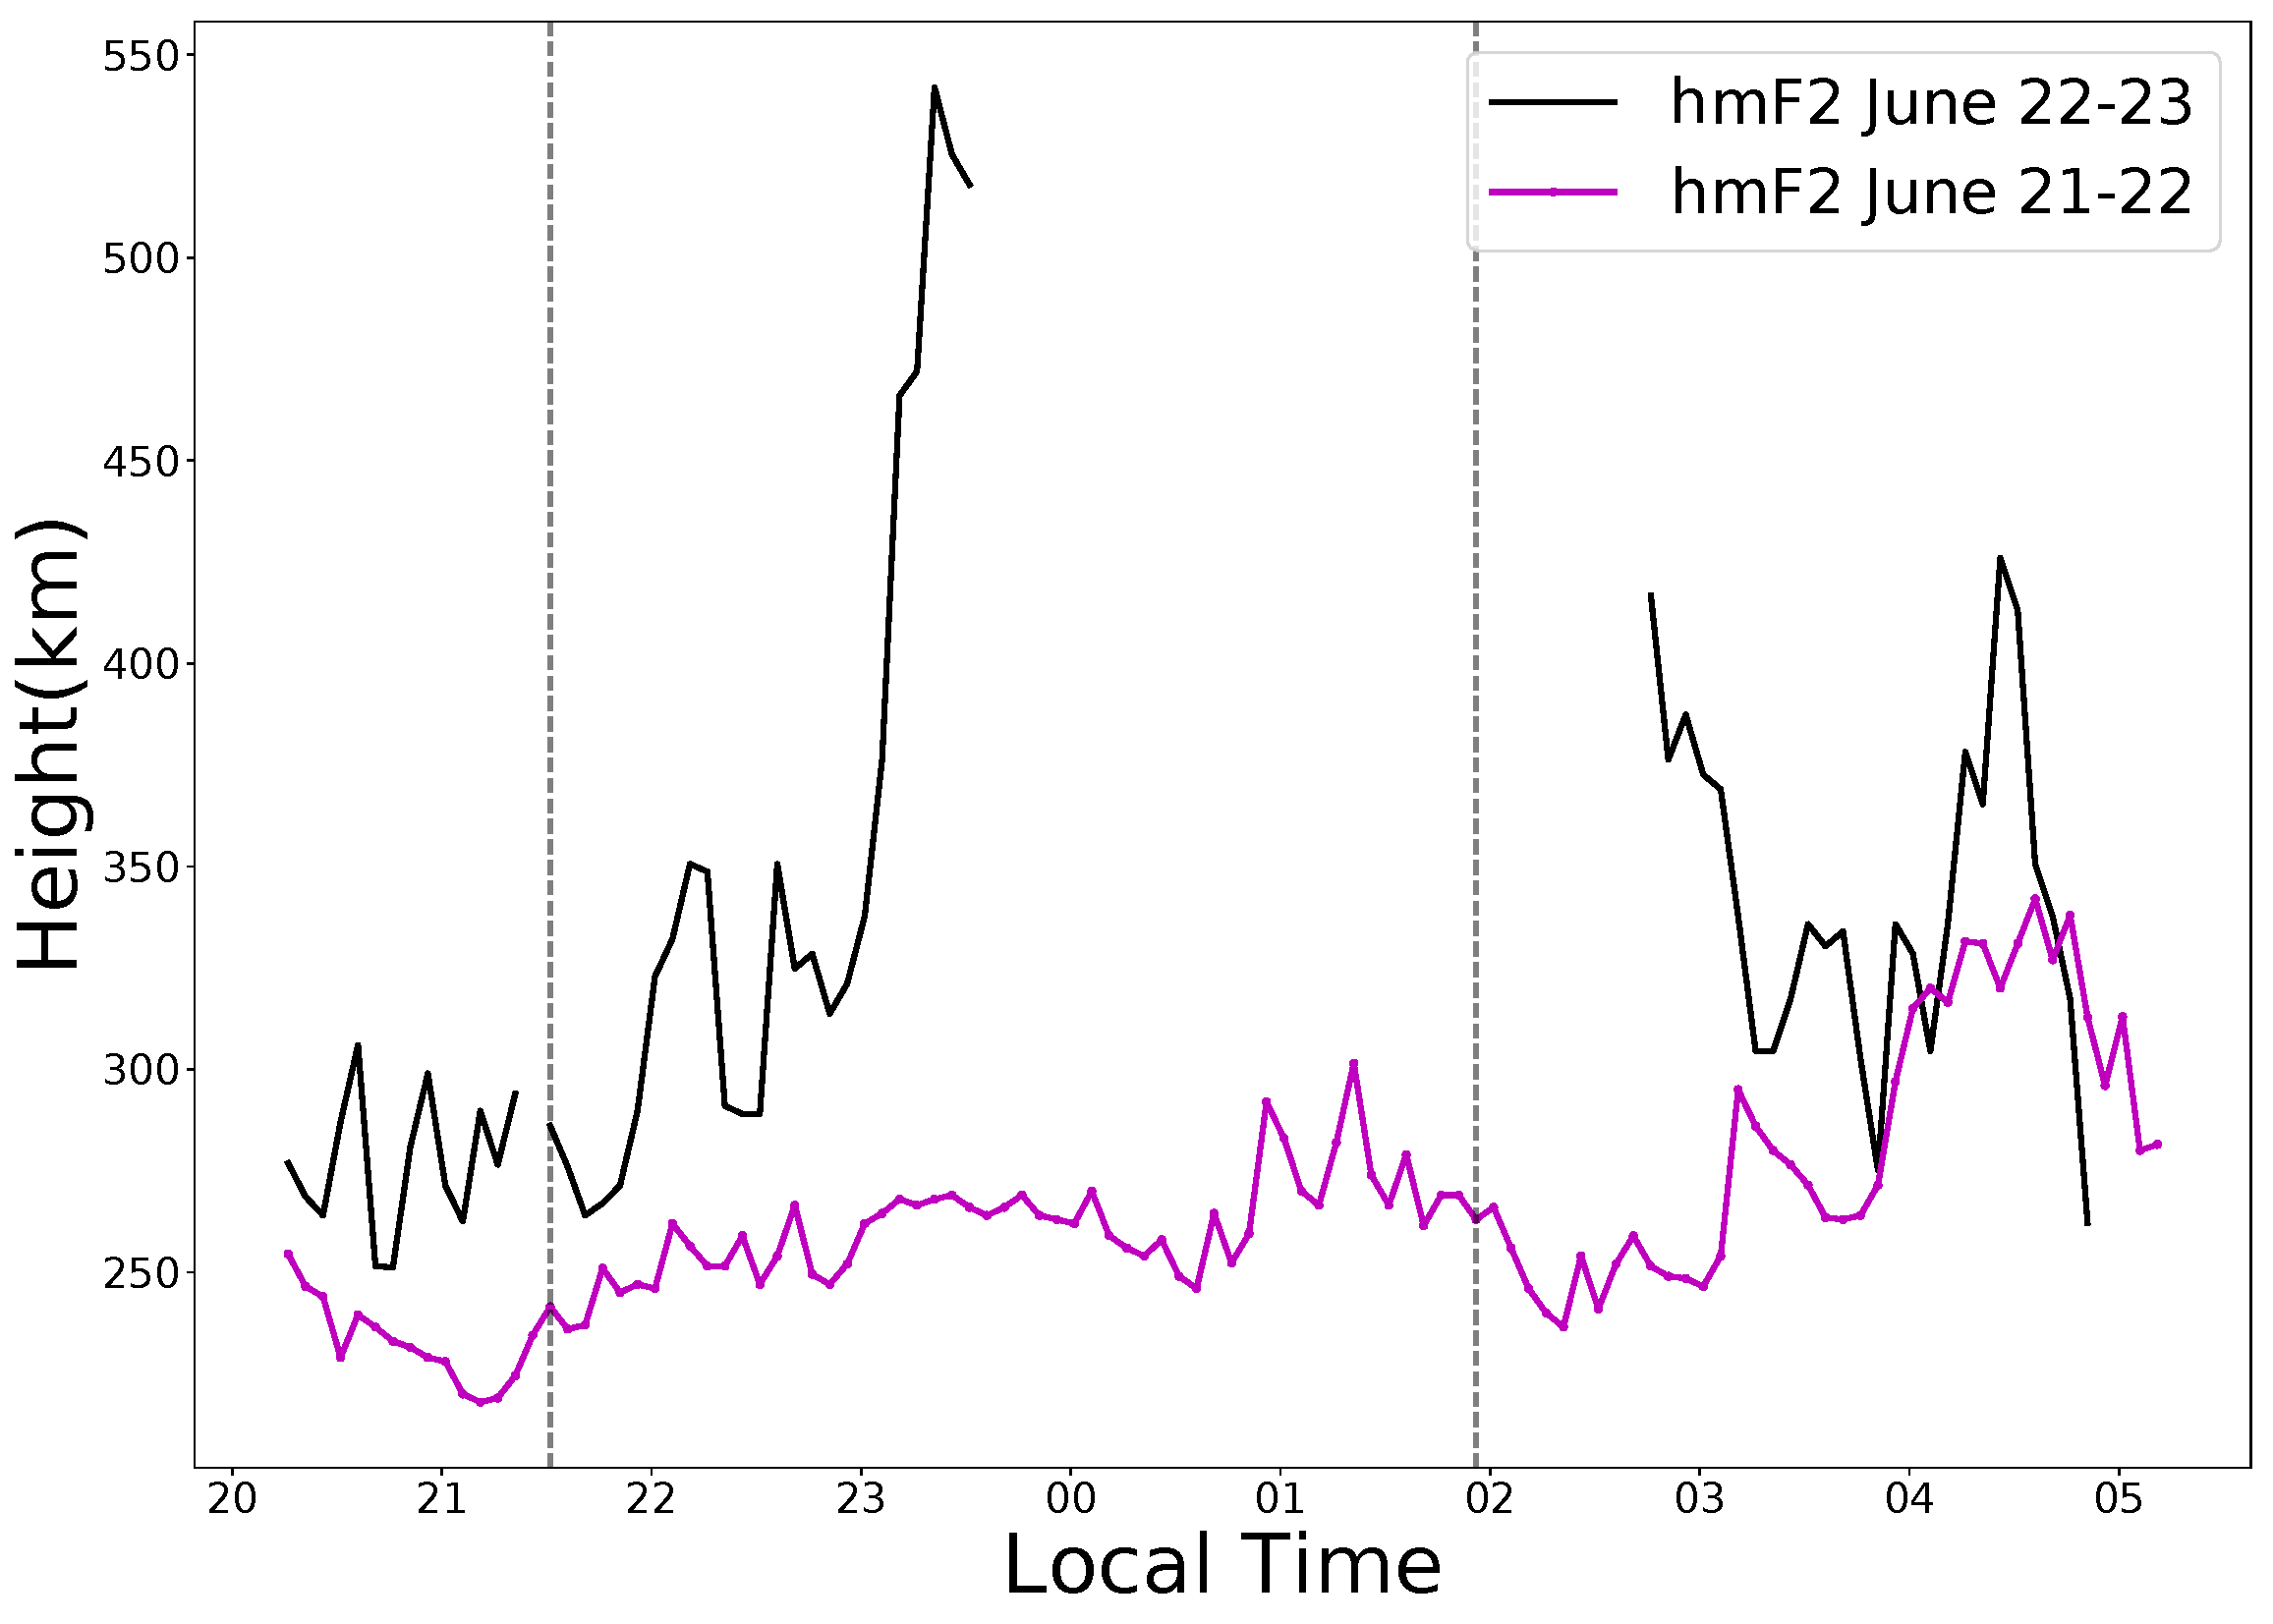
\includegraphics[width=20pc]{digi.pdf}
	\caption{ Digisonde measurements of hmF2 during the period of June 22, 2015 20 LT to 5 LT on June 23, 2015 are shown with the solid black line.
		hmF2 during the same time period (20 LT to 5 LT) by the same digisonde on June 21-22, 2015 on a geomagnetically quiet time are shown with the magenta line.
		The  HiT\&MIS observations were conducted between the two dashed vertical lines. Notice that hmF2 rises up before there is a signal loss on June 22-23 while hmF2 is almost constant (around 300 km) on June 21-22. The loss of signal on June 22-23, 2015 might be attributed to ionization caused by electron precipitation while the rise in hmF2 is a possible indicator of soft particle precipitation. 
	}
	\label{fig:digi}
\end{figure}

\section{Summary}
We have used ground-based spectral measurements to derive the energies and energy fluxes of precipitating electrons during an auroral event triggered by a G4 geomagnetic storm over Lowell, MA. Three different methods were compared based on non-linear minimization of $\chi^2$ in Equation \ref{eq:chi}. First, modeled brightnesses were compared with measurements to simultaneously derive energies and fluxes using the brightness method. Then, a similar technique where modeled brightness ratios were constrained with measurements to simultaneously derive the energies and fluxes was applied. Finally, modeled brightness ratios were compared with measurements to derive energies and then model brightnesses were constrained with measurements to derive fluxes using the hybrid method for comparison.  
%Third, energies and fluxes were simultaneously derived by constraining modeled brightness ratios with measured ratios using the one step ratio method. 
Results derived using the hybrid method (similar to methods used in \cite{rees_1974} and \cite{pallamraju_2011}) and the brightness method were in good agreement and reproduced the observed red and green line brightness profiles well. The derived energies ranged from 109 to 262 eV and the  energy fluxes ranged from 0.8 to 2.2 erg $\rm cm^{-2} s^{-1}$.
